\documentclass[oneside,final,14pt,a4paper]{extreport}

\usepackage{tempora} % Times New Roman alike font  
\usepackage{vmargin}
\setpapersize{A4}
\setmarginsrb{2.5cm}{2.2cm}{2.2cm}{2.2cm}{0pt}{10mm}{0pt}{13mm}
\usepackage{setspace}
\setstretch{1.5}
\usepackage{indentfirst}
\parindent=1.25cm

%%%%% ADDED TO SUPPORT TT BOLD FACES %%%%
\DeclareFontShape{OT1}{cmtt}{bx}{n}{<5><6><7><8><9><10><10.95><12><14.4><17.28><20.74><24.88>cmttb10}{}
\renewcommand{\ttdefault}{pcr}
%%%%% END %%%%%%%%%%%%%%%%%%%%%%%%%%%%%%% 

\usepackage{atbegshi,picture}
\usepackage[T1,T2A]{fontenc}
\usepackage{newtxtext}
\usepackage[utf8]{inputenc}

\usepackage[english]{babel}
\usepackage[backend=biber,style=ieee,autocite=inline]{biblatex}
\bibliography{ref.bib}
\DefineBibliographyStrings{english}{%
  bibliography = {References},}
\usepackage{blindtext}

\usepackage{pdfpages}
\newenvironment{bottompar}{\par\vspace*{\fill}}{\clearpage}
\usepackage{amsmath,amsfonts}
\usepackage{url}
\usepackage{amsthm}
\newtheorem{theorem}{Theorem}
\newtheorem{corollary}{Corollary}
\newtheorem{lemma}{Lemma}
\newtheorem{proposition}{Proposition}
\theoremstyle{definition}
\newtheorem{definition}{Definition}
\theoremstyle{remark}
\newtheorem*{remark}{Remark}
\theoremstyle{remark}
\newtheorem*{example}{Example}

\usepackage{float}
\usepackage{graphicx}
\graphicspath{{figs/}} %path to images
\usepackage{array}
\usepackage{multirow,array}
\usepackage{caption}
\usepackage{subcaption}
\usepackage{hyperref}
\hypersetup{colorlinks=true, linkcolor=black, citecolor=black}
\usepackage{paralist}
\usepackage{listings}
\usepackage{zed-csp}
\usepackage{fancyhdr}
\usepackage{csquotes}
\usepackage{color}
% \usepackage{anyfontsize}
% \usepackage{mathptmx}
% \usepackage{t1enc}

\usepackage{chngcntr}
\usepackage{upgreek} 
\usepackage{bm}
\usepackage{hyperref}
\usepackage{booktabs}
\usepackage{multirow}
\usepackage{longtable}
\usepackage[font=singlespacing, labelfont=bf]{caption}
%Hints
\newcommand\pic[1]{(Fig. \ref{#1})} %Ref on figure
\newcommand\tab[1]{(Tab. \ref{#1})} %Ref on table

\setlength{\headheight}{32.0976pt}
\usepackage{enumitem}
\newlist{inlinelist}{enumerate*}{1}
\setlist*[inlinelist,1]{%
  label=(\arabic*),
}

% \setcounter{secnumdepth}{4}
\captionsetup[table]{labelfont={normalfont}, name={TABLE}, labelsep={newline}}
\setlength{\parindent}{2em} 
\DeclareCaptionLabelSeparator{figSep}{.\quad}
\captionsetup[figure]{labelfont={normalfont}, name={Fig.}, labelsep=period}
\counterwithin{figure}{chapter}

% \usepackage{titlesec}
% \titleformat{\section}[hang]{\fontsize{20}{24}\selectfont\filcenter}{\Roman{section}}{1em}{}
% \titleformat{\subsection}[hang]{\itshape}{\Alph{subsection}.}{1em}{}[]
% \titleformat{\subsubsection}[runin]{\itshape}{\arabic{subsubsection})}{1em}{}[$:$]
% \titlespacing{\subsubsection}{1em}{1em}{1em}
% \titleformat{\paragraph}[runin]{\itshape}{\alph{paragraph})}{1em}{}[$:$\quad]
% \titlespacing{\paragraph}{2em}{1em}{1em}

\usepackage{placeins} % for \FloatBarrier
\usepackage{cases}
\usepackage{mathtools}
\usepackage{xcolor}
\usepackage[section]{algorithm}
\usepackage{algpseudocode}
\usepackage{tikz}
\usepackage{listings}
\usetikzlibrary{%
    decorations.pathreplacing,%
    decorations.pathmorphing%
}

\definecolor{dkgreen}{rgb}{0,0.6,0}
\definecolor{gray}{rgb}{0.5,0.5,0.5}
\definecolor{mauve}{rgb}{0.58,0,0.82}

\lstset { %
  captionpos=b,
  frame=tb,
  language=C++,
  showstringspaces=false,
  columns=flexible,
  % basicstyle={\small\ttfamily},
  basicstyle={\linespread{1}\ttfamily},
  numbers=left,
  numberstyle=\tiny\color{gray},
  keywordstyle=\color{blue},
  commentstyle=\color{dkgreen},
  stringstyle=\color{mauve},
  breaklines=true,
  breakatwhitespace=true,
  tabsize=4
}

\pagestyle{fancyplain}

\makeatletter
\newenvironment{breakablealgorithm}
  {% \begin{breakablealgorithm}
   \begin{center}
     \refstepcounter{algorithm}% New algorithm
     \hrule height.8pt depth0pt \kern2pt% \@fs@pre for \@fs@ruled
     \renewcommand{\caption}[2][\relax]{% Make a new \caption
       {\raggedright\textbf{\fname@algorithm~\thealgorithm} ##2\par}%
       \ifx\relax##1\relax % #1 is \relax
         \addcontentsline{loa}{algorithm}{\protect\numberline{\thealgorithm}##2}%
       \else % #1 is not \relax
         \addcontentsline{loa}{algorithm}{\protect\numberline{\thealgorithm}##1}%
       \fi
       \kern2pt\hrule\kern2pt
     }
  }{% \end{breakablealgorithm}
     \kern2pt\hrule\relax% \@fs@post for \@fs@ruled
   \end{center}
  }
\makeatother

% Remember section title
\renewcommand{\chaptermark}[1]%
	{\markboth{\chaptername~\thechapter~--~#1}{}}

% subsection number and title
\renewcommand{\sectionmark}[1]%
	{\markright{\thesection\ #1}}

\rhead[\fancyplain{}{\bf\leftmark}]%
      {\fancyplain{}{\bf\thepage}}
\lhead[\fancyplain{}{\bf\thepage}]%
      {\fancyplain{}{\bf\rightmark}}
\cfoot{} %bfseries


\newcommand{\dedication}[1]
   {\thispagestyle{empty}
     
   \begin{flushleft}\raggedleft #1\end{flushleft}
}

% Taken from https://cremeronline.com/LaTeX/minimaltikz.pdf
\newcommand{\base}[2]{
  % triangle below circle
  \draw[black, thick] (#1 - 0.3, #2 - 0.5) -- (#1 - 0.1, #2 -0.2);
  \draw[black, thick] (#1 + 0.1, #2 - 0.2) -- (#1 + 0.3, #2 -0.5);

  % base lines
  \draw[black, thick] (#1 - 0.5, #2 - 0.5) -- (#1 + 0.5, #2 - 0.5);
  % dashes
  \draw[black,line width=.5pt,interface](#1 - 0.5, #2 - 0.5)--(#1 + 0.5, #2 - 0.5);
  % circle
  \draw [black, thick,fill=white] (#1, #2) circle [radius=0.2];
}

\newcommand{\drawpointmass}[3][0]{
  % semitransparent circle
  \draw [fill=#1, fill opacity=0.2, draw=#1!40] (#2, #3) circle [radius=0.4];
  % circle
  \draw [black, thick, fill=white] (#2, #3) circle [radius=0.2];
}

\newcommand{\drawpointmasssimple}[3][0.2]{
  % circle
  \draw [black, thick, fill=white] (#2, #3) circle [radius=#1];
}

\newcommand{\drawdot}[3][0.05]{
  % circle
  \draw [black, thick, fill=black] (#2, #3) circle [radius=#1];
}

\newcommand{\gripper}[4]{
  % Adjoint lines
  \draw[black, ultra thick](#1, #2) -- (#1 - #4 / 2 + #2 / 2, #2 + #3 / 2 - #1 / 2);
  \draw[black, ultra thick](#1, #2) -- (#1 + #4 / 2 - #2 / 2, #2 - #3 / 2 + #1 / 2);
  % Parallel lines
  \draw[black, ultra thick]
  (#1 - #4 / 2 + #2 / 2, #2 + #3 / 2 - #1 / 2) -- 
  (#1 - #4 / 2 + #2 / 2 + #3 - #1, #2 + #3 / 2 - #1 / 2 + #4 - #2);
  \draw[black, ultra thick]
  (#1 + #4 / 2 - #2 / 2, #2 - #3 / 2 + #1 / 2) -- 
  (#1 + #4 / 2 - #2 / 2 + #3 - #1, #2 - #3 / 2 + #1 / 2 + #4 - #2);
}

\newcommand{\rectangle}[6]{
  \draw[black, ultra thick](#1, #2) -- (#3, #4);
  \draw[black, ultra thick](#3, #4) -- (#5, #6);
  \draw[black, ultra thick](#1, #2) -- (#1 + #5 - #3, #2 + #6 - #4);
  \draw[black, ultra thick](#1 + #5 - #3, #2 + #6 - #4) -- (#5, #6);
}

\newcommand{\RNum}[1]{\uppercase\expandafter{\romannumeral #1\relax}}

\newcommand{\SE}[1][3]{\text{SE}(#1)}

\newcommand{\SO}[1][3]{\text{SO}(#1)}

\title{Feedback control over constrained robotic systems through the Udvadia-Kalaba approach}
\author{Ilia Milioshin}

\begin{document}
% \includepdf[pages=-]{title.pdf}
\maketitle
\tableofcontents
% \listoftables
% \listoffigures
\newpage

% \begin{abstract}

The cooperation of robotic systems, particularly when constrained by shared 
objects, presents a significant challenge in various domains. Previous 
methods, such as models with pre-existing constraints or the 
Karush-Kuhn-Tucker (KKT) approach, suffer from computational complexity and 
prioritization issues. This research solves these limitations by proposing 
a novel methodology based on the Udwadia-Kalaba approach. 
The objective is to enhance control and collaboration of robots using 
advanced tools like MuJoCo, Pinocchio, and ProxSuite. The method integrates 
physical grounding and simplicity, allowing manual fine-tuning of 
constraint priorities and achieving improved computational speed. 
Experimental results demonstrate significant improvements in efficiency, 
accuracy, and adaptability in robotic operations. These advancements suggest 
potential for increased productivity and optimized performance in 
industrial and real-life applications, laying the way for further 
robotics technology developments. For example, 

\end{abstract}
\setcounter{page}{1}
% set manually the number, from which Chapter 1 starts!
% Why do we put 7 in this case?
% Title page - page 1
% Contents - page 2, page 3
% List of tables - page 4
% List of figures - page 5
% Abstract - page 6
% Chapter 1 - page 7
% In your thesis the counter number can be different, please count carefully and insert the corresponding number.

\chapter{Introduction}
\label{chap:intro}
% \chaptermark{Optional running chapter heading}

The advancement of microelectronics and sensor technologies has catalyzed a 
widespread integration of robotic systems into various domains. Manipulators, 
delivery robots, and flying drones have become ubiquitous, presenting developers 
and researchers with novel challenges in terms of robustness, adaptiveness, and 
synchronization. Among these challenges, synchronization stands out as a critical 
issue, especially given the proliferation and increasing complexity of such systems. 
 In real-world applications, synchronization of robotic systems is crucial across 
various industries. For instance, in manufacturing assembly lines, synchronized 
robots ensure smooth production flow and maximize throughput. Similarly, in 
warehouse logistics, coordinated robotic systems optimize order fulfillment times 
and enhance overall productivity. Furthermore, collaborative robotics scenarios in 
construction projects benefit from synchronized robotic systems for tasks like 
concrete pouring and steel beam placement, improving efficiency and minimizing 
delays. A common challenge in this realm involves effectively controlling robots constrained 
by a shared object. This paper proposes a straightforward methodology to address 
such problems through the Udwadia-Kalaba\cite{UdwadiaKalabaApproach} approach.

This proposed methodology gains particular significance within the context of modern 
physics simulation, derivation, and optimization libraries. These tools offer 
substantial computational speed, enabling efficient problem-solving. In this article, 
we leverage MuJoCo\cite{MuJoCo}, Pinocchio\cite{Pinocchio}, and ProxSuite\cite{CvxPy} 
for simulation, robotic dynamics computation, and optimization, respectively. 
Pinocchio, in particular, emerges as a key tool for computing the dynamics of robotic 
systems. However, its limitation to open-loop physics models poses challenges for 
controlling and synchronizing multiple robots.

Previous solutions have often involved constructing models with pre-existing 
constraints or employing the KKT (Karush-Kuhn-Tucker) approach. However, these 
methods suffer from computational complexity and issues with constraint 
prioritization. The proposed methodology combines the strengths of both approaches, 
integrating physical grounding from the former and simplicity of application from 
the latter. Notably, it allows for manual fine-tuning of constraint priorities and 
boasts superior computational speed through auto code generation. 

The implementation of the proposed methodology demonstrates significant advancements 
in the control and synchronization of robotic systems constrained by shared objects. 
Through the integration of robust physics simulation, precise robotic dynamics 
computation, and efficient optimization techniques, the method achieves remarkable 
outcomes across various simulation experiments. By leveraging 
advanced simulation, computation, and optimization techniques, the method has 
improved levels of efficiency, accuracy, and adaptability in robotic operations, 
paving the way for further advancements in automation and robotics technology.

In subsequent chapters, we delve deeper into various aspects of the proposed method. 
Chapter \ref{chap:lr} provides an exhaustive review of recent literature, 
highlighting the existing landscape of solutions and their limitations. 
Chapter \ref{chap:met} elucidates the methodology underlying the proposed approach, 
offering insights into its theoretical underpinnings. Implementation details and 
code snippets are presented in Chapter \ref{chap:impl}, demonstrating the practical 
application of the method. Chapter \ref{chap:eval} undertakes a comparative 
analysis, pitting technique against established methods to gauge its efficacy. 
Finally, Chapter \ref{chap:conclusion} summarizes findings, discusses 
implications, and outlines avenues for future research.

\chapter{Literature Review}
\label{chap:lr}
% \chaptermark{Second Chapter Heading}

The control of the interacting physical systems is a challenging 
task. There are few problems that should be solved to achieve the 
high efficiency and precision in the aforementioned problem. They 
are the following: the right mathematical model selection, the 
unified methodology for defining the interaction, and the well-defined 
control error. The first point is necessary to cover a wide range 
of physical systems. The second one is crucial to work with 
different mechanical connections. Finally, the last one is needed 
to stability and robustness analysis. 

This literature review covers all these subproblems and explores them
from the point of view of the work of Firdaus Udwadia and Robert Kalaba 
\cite{UdwadiaKalabaApproach}. The section \ref{sec:math_model} considers 
a mathematical models that utilized in the recent studies. The 
\ref{sec:interaction_def} part reviews a rigorous methodology to define 
how physical systems can affect each other. The section \ref{sec:control_error} 
explores the previous research in control error defining and analysis 
on different manifolds.

The articles were selected to demonstrate a solid ground why some methods 
had been preferred in this study. Some of the papers were chosen 
to reference for theoretical background that was not included in this 
paper. Other articles had been reviewed for shown an existing techniques.

\section{The mathematical model} \label{sec:math_model}

This section contains review of existing mathematical models for physical 
systems. Moreover, this piece has a comparison of them in terms of numerical 
integration convenience and simplicity of defining the initial conditions. 
It is necessary to clarify that from now this study considers only systems 
of rigid body with only inner stiffness. The detailed explanation of 
such choice will be conduct later in the Chapter \ref{chap:met}.

Firstly, lets consider the most popular model. The articles 
\cite{UdwadiaKalabaApproach}, \cite{AppOfUdwadiaKalabaApproach} and 
\cite{UnifiedFrameworkOfRobotControl} relies on it. Usually it is 
called the canonical manipulator equation. The model can be formulated 
as 

\begin{equation} \label{eqn:can_man_equation}
    M(\mathbf{q})\ddot{\mathbf{q}} + 
    C(\mathbf{q}, \dot{\mathbf{q}}) \dot{\mathbf{q}} + 
    g(\mathbf{q}) = 
    \boldsymbol{\tau}
\end{equation}

where $M(\mathbf{q})$ is known as inertia matrix, $C(\mathbf{q}, \dot{\mathbf{q}})$ 
is Centrifugal-Coriolis matrix, $g(\mathbf{q})$ is a gradient
of potential forces, and $\mathbf{q}$, $\boldsymbol{\tau}$ are generalized 
coordinates and torques respectively. This equation will be explored in details 
in the next Chapter \ref{chap:met}.

Conversely, Udwadia \cite{ConstHamiltonSys} utilized a Hamiltonian view of the 
problem. The equations are following, 

\begin{equation}
    \label{eqn:ham_eqns}
    \begin{cases}
        \dot{\mathbf{q}} = \frac{\partial \mathcal{H}}{\partial \mathbf{p}} \\
        \dot{\mathbf{p}} = -\frac{\partial \mathcal{H}}{\partial \mathbf{q}}
    \end{cases}
\end{equation}

where $\mathbf{q}$, $\mathbf{p}$, and $\mathcal{H}$ are generalized coordinates,
generalized momentum, and Hamiltonian respectively.

The aforementioned equations are proven to be equivalent. Thus, both models 
can be utilized for achieving the main goal. However, the crucial difference 
lies in the another plane. 

In the vast majority of cases the both differential equations can be solved 
analytically. Therefore, it is necessary to use the numerical methods. The 
equation (\ref{eqn:can_man_equation}) has second time derivative. It forces 
to construct proper state variable for numerical integration. In the opposite 
the Hamiltonian equations (\ref{eqn:ham_eqns}) has only first derivative. Hence, 
the usage of it is simpler. However, the definition of initial conditions is harder.
Nevertheless, the mentioned problem are already solved. So, choice of model 
fully lies on the specific of discussed task. 

The most of reviewed papers relies on the canonical model 
(\ref{eqn:can_man_equation}). Therefore, this research will utilize this equation 
too.

\section{The methodology to defining interaction} \label{sec:interaction_def}

The second crucial point in this paper is a definition of interaction between 
systems. This piece considers how it can be achieved, and which methodology 
is better in the context of discussed question. The important remark of this 
section that only interaction via rigid bodies will be consider below.

The first discussed approach is analyzed in \cite{OptimizationBasedLocomotionPlanning} 
and \cite{WholeBodyControlForm}. These articles propose to use a 
a force cone to define an contact between a physical system 
and solid surface. The actuation force can be formulated as 

\begin{equation}
    \label{eqn:force_cone}
    \pmb{\lambda} = \sum_{i=1}^{N_d} \beta_i (\mathbf{n} + \mu \mathbf{d}_i), 
    \: \beta_i \ge 0
\end{equation}

where $\mathbf{n}$ is a normal force, $\mathbf{d}_i$ is a tangent to contact 
vector, $\mu$ is the Coulomb friction coefficient, and $N_d$ is a amount
of used tangent vectors. This contact force later can be translated to 
joint space via respective jacobian - $J^T(\mathbf{q})$.

Using this approach it is possible to emulate an interaction between 
physical systems via rigid body. It can be achieved by defining the motion 
of connection body through force acting on it. However, this method cannot 
guaranty a stability. Moreover, constructing a feedback loop in this case is 
not trivial task. 

The next straight forward solution is initially impose an interaction inside 
to mathematical model. In the discussed case it can be achieved by writing 
the $M(\mathbf{q})$, $C(\mathbf{q}, \dot{\mathbf{q}})$, and $g(\mathbf{q})$ 
in equation (\ref{eqn:can_man_equation}) as formulation of closed-loop system. 
Thus, the advantage of this method is unnecessary of stabilization, because 
it is guaranteed by a model itself. Futhermore, this formulation can be 
used with a great range of control techniques. However, \cite{BodyDynWithClosedLoop} 
demonstrates a lower computation speed with comparison to 
open-loop algorithms \cite{Pinocchio}. Moreover, proposed closed-loop 
version requires a predefined description of a whole system. Thus, it cannot 
be used in the realtime in the dynamic environment.

Finally, the third approach is defining a right constraint. In this study the action 
of the rigid body on connected systems can be described by holonomic constraint. 
It can be formulated as 

\begin{equation}
    \label{eqn:holonom_const}
    \varphi (\mathbf{q}, t) = 0
\end{equation}

Further this equation can be used in KKT (Karush-Kuhn-Tucker) technique to 
rigorous define system with imposed constraints. Moreover, using the equation
(\ref{eqn:holonom_const}) it is straight forward to construct a stabilization 
mechanism. As instance, the Baumgarte's approach can be used with KKT method 
to achieve this goal. Nevertheless, this study does not rely on aforementioned 
technique (KKT), instead it utilized the Udwadia-Kalaba approach. Details are 
shown in the Chapter \ref{chap:met}.

\section{Control error} \label{sec:control_error}

The last crucial subproblem is rigorous defining of control error for ensure 
stabilization. Especially, it is important in the context of chosen type of 
interaction. Therefore, this section reviews how to calculate the discrepancy 
between the current system state and desired one in the form of the equation 
(\ref{eqn:holonom_const}). 

The previous studies \cite{SlidingOnManifoldsQuat,GeomControlQuadSE3,
RigidBodyAttCon,OutFeedbackStabForOrbRob,ANonlinearObserverUsingPose} 
concentrates on computing pose difference in space. The majority 
\cite{GeomControlQuadSE3,RigidBodyAttCon,OutFeedbackStabForOrbRob,
ANonlinearObserverUsingPose} of source explores problem through utilizing 
rotations matrices. On the other hand \cite{SlidingOnManifoldsQuat} uses 
a quaternions for achieving the goal. Let's compare these solutions.

The \cite{SlidingOnManifoldsQuat} states the advantage of quaternions on 
the rotations matrix. This research shows that proposed method achieves 
the \emph{exponential asymptotic stability} against \emph{almost global 
stability} of techniques from \cite{GeomControlQuadSE3,RigidBodyAttCon}.
Futhermore, the quaternion-based method in discussed study presents the 
superiority on the analogous ones. The authors proves that their technique 
avoids the unwinding phenomenon, i.e. error converges to zero by shortest 
path in $\mathbb{S}^3$.

The solution via utilizing the rotations matrices is presented in 
\cite{GeomControlQuadSE3,RigidBodyAttCon,OutFeedbackStabForOrbRob,
ANonlinearObserverUsingPose}. However, in aforementioned quaternion-based 
approach shows that basing on such structure methods has disadvantage. 
The naive error computation via matrices is calculation of dot product 
between base vectors of current and desired orientation. As mentioned 
above this approach can achieve only \emph{almost global stability}. 
Nevertheless, studies \cite{OutFeedbackStabForOrbRob, ANonlinearObserverUsingPose} 
relies on deep topology analysis of $SE(3)$ group. These research uses 
a Lie theory to construct a right discrepancy between attitudes. In 
the Chapter \ref{chap:met} the \emph{exponential convergence} of method 
based on articles above is presented.

\chapter{Methodology}
\label{chap:met}

This chapter will present a detailed explanation of the principles underlying the 
proposed methodology. The section \ref{sec:rigid_body_and_const} offers a concise 
overview of rigid-body systems and constraints that can be imposed on them.
The next section \ref{sec:udwadia_kalaba_app} introduces the Udwadia-Kalaba 
approach and physical principles that stays behind it. Further in Section 
\ref{sec:def_rigid_body_const}, this technique is applied to solve the discussed 
problem. Then Section \ref{sec:control_through_udwadia} use the Udwadia-Kalaba 
approach to construct a control law. Finally, Section 
\ref{sec:task_prioritization} contains thoughts about prioritization constraint 
task over control one. 

\section{Rigid-body systems and constraints} 
\label{sec:rigid_body_and_const}

The most common class of physical systems that can be observed in the real life 
cases is the rigid-body one. Some examples of such systems are demonstrated in 
Figure \ref{fig:examples_of_rig_sys}. The key feature of rigid-body systems 
is non-deformable parts that forms it. With these limitations only an 
inner stiffness can be described.

\begin{figure}[H]
    \centering
    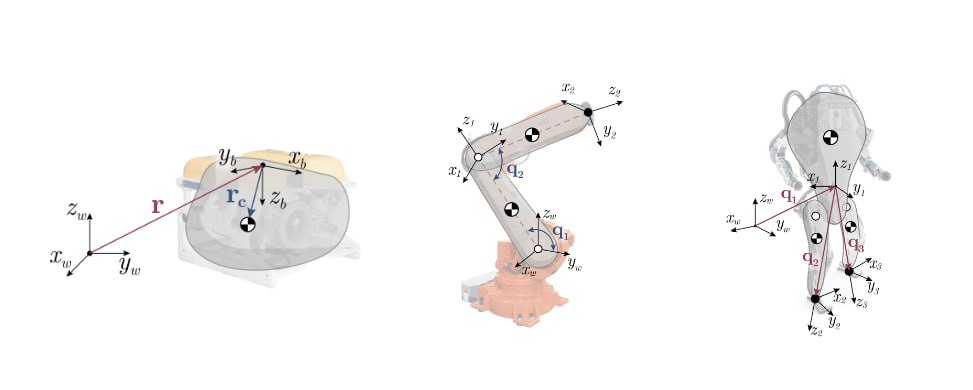
\includegraphics[scale=0.5]{figs/rigid_body_systems.png}
    \caption{Examples of rigid-body systems}
    \label{fig:examples_of_rig_sys}
\end{figure}


Nevertheless, the mathematical tools to work with rigid-body systems was introduced 
in \RNum{18}-th century by Newton and Euler works. Using this approach it is easy 
to formulate a set of deferential equations that describes the system behavior.
However, in this study the another (more convenient) technique is utilized. It is 
called the least action principle. The formulation is the following equation

\begin{equation}
    \min_{\mathbf{q}} \quad 
    \int_{t_1}^{t_2} L(\mathbf{q}(t), \mathbf{v}(t), t) dt
    \label{eqn:least_act_principle}
\end{equation}

where $L$ is Lagrangian of the system, and $\mathbf{q}$, $\mathbf{v}$ are 
functions of the generalized coordinates and velocities respectively. The solution 
of the variational problem (\ref{eqn:least_act_principle}) is the Euler-Lagrange 
differential equations. The solution through utilizing the Lagrangian can be 
easily generalized to all rigid-body systems. This generalization is aforementioned 
the canonical manipulator equation (\ref{eqn:can_man_equation}). 

In this chapter the convenient representation of this equation is used. The main 
idea of rewriting is combination of the inertial forces with non-inertial ones.

\begin{equation}
    M \dot{\mathbf{v}} = \mathbf{Q}
    \label{eqn:can_man_eqn_simple}
\end{equation}

In the above equation $\mathbf{Q} = 
-C(\mathbf{q}, \mathbf{v}) \dot{\mathbf{q}} - g(\mathbf{q}) + 
\boldsymbol{\tau}$, $M \succcurlyeq 0$ is inertia matrix, $C$ is Centrifugal-Coriolis 
matrix, $g$ is gradient of conservative forces. The dependency from coordinates and 
velocities is amended for convenience. In the most generalized case 
$\dim{\mathbf{q}} = n_q \neq n_v = \dim{\mathbf{v}}$.

The aforementioned description is applicable for open and closed loop systems. 
The closed one is described in Figure \ref{fig:rigid_coupling}. However, 
as mentioned above utilizing only equation \ref{eqn:can_man_eqn_simple} to handle 
such system is not efficient. Thus, the approach via constraints described
by equation (\ref{eqn:holonom_const}) is more preferable. It can be inserted in 
(\ref{eqn:least_act_principle}), which leads to the following variational problem, 

\begin{equation}
    \min_{\mathbf{q}} \quad 
    \int_{t_1}^{t_2} [L(\mathbf{q}(t), \mathbf{v}(t), t) - 
    \pmb{\lambda}^T \varphi(\mathbf{q}(t), t)]dt
    \label{eqn:least_act_principle_const}
\end{equation}

The solution the above equation can be expressed in terms of the KKT matrix in 
the following way, 

\begin{equation}
    \begin{bmatrix}
        M & J^T \\
        J & 0 \\
    \end{bmatrix}
    \begin{bmatrix}
        \dot{\mathbf{v}} \\
        -\pmb{\lambda}
    \end{bmatrix} = 
    \begin{bmatrix}
        \mathbf{Q} \\
        -\dot{J} \mathbf{v}
    \end{bmatrix}, \:
    J = \frac{\partial \boldsymbol{\varphi}}{\partial \mathbf{q}}
    \label{eqn:kkt_solution}
\end{equation}

The downside of the equation (\ref{eqn:kkt_solution}) is that it does not support 
non-holonomic constraints generally. This type of constraints can be defined as 

\begin{equation}
    \varphi(\mathbf{q}, \mathbf{v}, t) = 0
    \label{eqn:non_holonomic_const}
\end{equation}

Therefore, the dependency from generalized velocity makes the KKT approach not 
applicable. The handle of such constraints is crucial for defining a control. 
Hence, it is necessary to use another technique.

\section{The Udwadia-Kalaba approach} \label{sec:udwadia_kalaba_app}

The main differences of the Udwadia-Kalaba approach from the method mentioned 
above are the another view on constraints, and utilizing different physical 
principle.

Let's start from reviewing the constraints form in the discussed technique. It 
can be derived from holonomic and non-holonomic type by differentiating over time, 
and transforming to an affine form. The general equation is the following 

\begin{equation}
    A(\mathbf{q}, \mathbf{v}, t) \dot{\mathbf{v}} = 
    \mathbf{b}(\mathbf{q}, \mathbf{v}, t)
    \label{eqn:affine_const}
\end{equation}

The above equation can be used in the Gauss least constraint principle. For further 
convenience the arguments of matrix functions is amended. It leads to the 
following optimization problem:

\begin{equation}
    \begin{aligned}
        \min_{\dot{\mathbf{v}}} \quad &
        [\dot{\mathbf{v}} - \mathbf{a}]^T M [\dot{\mathbf{v}} - \mathbf{a}] \\
        \textrm{s.t.} \quad &
        A \dot{\mathbf{v}} = \mathbf{b} \\
        &
        \mathbf{a} = M^{-1} \mathbf{Q}
    \end{aligned}
    \label{eqn:gauss_least_const}
\end{equation}

This optimization can be solved analytically as Ferdaus Udwadia and Robert Kalaba 
demonstrated \cite{UdwadiaKalabaApproach}. This solution is shown below.

\begin{equation}
    \dot{\mathbf{v}} = 
    \mathbf{a} + M^{-1 / 2}(A M^{-1 / 2})^+ (\mathbf{b} - AM^{-1} \mathbf{Q})
    \label{eqn:udwadia_kalaba_sol}
\end{equation}

where $[\cdot]^+$ is the Moore-Penrose inverse, and 
$M^{\pm 1 / 2} = W \Lambda^{\pm 1 / 2} W^T$, $W$ is the orthogonal matrix 
of eigen vectors. 

In case of positive semi-definiteness of $M$ the equation 
(\ref{eqn:udwadia_kalaba_sol}) is not applicable because $M^{-1}$, 
$M^{-1 / 2}$ cannot exist. The Firdaus Udwadia and Aaron Schutte demonstrates 
\cite{EquationsOfMotionConst} a methodology to bypass this problem by 
replacing $M$, and $\mathbf{a}$ by the following quantities respectively

\begin{equation}
    \begin{aligned}
        M_A = M + A^+ A \succ 0 \\
        \mathbf{a}_A = M_A^{-1} \mathbf{Q}
    \end{aligned}
    \label{eqn:another_mass_matrix}
\end{equation}

Utilizing the mentioned quantities it is possible to define constraints 
force over the wide range of rigid-body systems. These forces can be 
expressed in the following manner 

\begin{equation}
    \mathbf{Q}_C = M^{1 / 2} (A M^{-1 /2})^+(\mathbf{b} - AM^{-1} \mathbf{Q})
    \label{eqn:constraint_forces}
\end{equation}

Hence, the Udwadia-Kalaba approach is applicable for emulation of 
rigid body constraint in computation easily. Only the problem with rigorous 
defining $A$ and $\mathbf{b}$ remains.

\section{Defying rigid body constraint}
\label{sec:def_rigid_body_const}

As mentioned above the discussed coupling between physical systems is created 
by some rigid body. This type of mathematical object can be described by the 
following identity for any two points

\begin{equation}
    \| \mathbf{r}_A(t) - \mathbf{r}_B(t) \| \equiv \text{const}
    \label{eqn:rigid_body_axiom}
\end{equation}

From the above equation kinematic laws can be directly derived. For further 
investigations it is necessary to introduce a point's velocity of the rigid 
body

\begin{figure}[H]
    \centering
    \begin{tikzpicture}[
        media/.style={font={\footnotesize\sffamily}},
        interface/.style={
            % The border decoration is a path replacing decorator.
            % For the interface style we want to draw the original path.
            % The postaction option is therefore used to ensure that the
            % border decoration is drawn *after* the original path.
            postaction={draw,decorate,decoration={border,angle=-45,
            amplitude=0.3cm,segment length=2mm}}},
        ]
        % Object
        \draw [black, thick] plot [smooth cycle] coordinates {
            (2.7, 2.2) (3.5, 3.4) (4.3, 3.8) (4.1, 2.6) (6.0, 2.0) (6.0, 1.3) (3.5, 1.0)
        };
        \draw[media] (4.6, 3.7) node {\Large $\boldsymbol \Sigma$};

        % p_A
        \draw[black, ->, dashed](4.000, -1.167) -- (2.800 + 0.02, 2.033 - 0.07);
        \draw[media] (3.1, 0.40) node {\large $\mathbf{r}_A$}; 
        % p_B
        \draw[black, ->, dashed](4.000, -1.167) -- (6.000 - 0.05, 1.833 - 0.06);
        \draw[media] (5.3, 0.2) node {\large $\mathbf{r}_B$}; 
        % p_AB
        \draw[black, ->, dashed](2.800, 2.033) -- (6.000 - 0.1, 1.833 + 0.05);
        \draw[media] (4.4, 2.2) node {\large $\mathbf{r}_{AB}$};

        % world frame
        \draw[black, ->](4.000, -1.167) -- (5.102, -1.273);
        \draw[black, ->](4.000, -1.167) -- (4.000, 0.000);
        \draw[black, ->](4.000, -1.167) -- (3.318, -1.363);
        \drawdot{4.000}{-1.167}
        \draw[media] (4.400, -0.867) node {\Large $\mathcal{W}$}; 
        \draw[media] (5.260, -1.288) node {\large $y$}; 
        \draw[media] (4.000, 0.200) node {\large $z$}; 
        \draw[media] (3.172, -1.406) node {\large $x$}; 

        % A frame
        \draw[black, ->](2.800, 2.033) -- (3.889, 1.628);
        \draw[black, ->](2.800, 2.033) -- (2.800, 3.029);
        \draw[black, ->](2.800, 2.033) -- (2.133, 1.289);
        \drawdot{2.800}{2.033}
        \draw[media] (3.100, 2.433) node {\Large $\mathcal{A}$}; 
        \draw[media] (4.045, 1.570) node {\large $y$}; 
        \draw[media] (2.800, 3.230) node {\large $z$}; 
        \draw[media] (1.990, 1.130) node {\large $x$}; 

        % B frame
        \draw[black, ->](6.000, 1.833) -- (6.943, 2.371);
        \draw[black, ->](6.000, 1.833) -- (5.515, 2.850);
        \draw[black, ->](6.000, 1.833) -- (5.318, 1.637);
        \drawdot{6.000}{1.833}
        \draw[media] (5.600, 1.433) node {\Large $\mathcal{B}$};
        \draw[media] (7.078, 2.448) node {\large $y$};
        \draw[media] (5.446, 3.100) node {\large $z$};
        \draw[media] (5.172, 1.594) node {\large $x$};

        % Draw first manipulator
        \draw[black, ultra thick](0, 0) -- (0.5, 1.8);
        \draw[black, ultra thick](0.5, 1.8) -- (2.5, 2.2);
        % Gripper
        \gripper{2.5}{2.2}{3.3}{2.36}
        % Draw second point mass
        \drawpointmasssimple{0.5}{1.8}
        \base{0}{0}
        \draw[media] (-0.3, 0.6) node {\Large $\mathbf{S}_1$};
        
        % % Draw the second manipulator
        \draw[black, ultra thick](8, 1) -- (7.577, 3.577);
        \draw[black, ultra thick](7.577, 3.577) -- (6.177, 2.177);
        % % Gripper
        \gripper{6.177}{2.177}{5.6}{1.6}
        % % Draw second point mass
        \drawpointmasssimple{7.577}{3.577}
        \base{8}{1}
        \draw[media] (8 + 0.4, 1 + 0.5) node {\Large $\mathbf{S}_2$};
    \end{tikzpicture}
    \caption{Rigid body ($\boldsymbol{\Sigma}$) coupling with frames}
    \label{fig:coupling_rigid_body}
\end{figure}

\begin{equation}
    \begin{aligned}
        \boldsymbol{\upsilon}_B = \boldsymbol{\upsilon}_A + 
        \boldsymbol{\omega}_A \times \mathbf{r}_{AB} \\
        \boldsymbol{\omega}_A = \boldsymbol{\omega}_B 
        = \boldsymbol{\omega}_{\Sigma}
    \end{aligned}
    \label{eqn:motion_of_rig_body}
\end{equation}

Equation (\ref{eqn:motion_of_rig_body}) describes motion of points, which 
shown in the Fig. {\ref{fig:coupling_rigid_body}}. $\boldsymbol{\omega}_X$ 
denotes the angular velocity of some \emph{fixed frame} with the origin at $X$.
Further in this chapter the below notation is used for for attitude (member of $\SE$) 
description:

\begin{equation}
    T_{\mathcal{W}}^{\mathcal{A}} = 
    \begin{bmatrix}
        R^{\mathcal{A}}_{\mathcal{W}} & \mathbf{p}_{\mathcal{A}} \\
        \mathbf{0} & 1
    \end{bmatrix}
    \in \SE
    \label{eqn:se_3_element}
\end{equation}

where $R^{\mathcal{A}}_{\mathcal{W}} \in \SO$ represents basis of $\mathcal{A}$ 
in $\mathcal{W}$, and $\mathbf{p}_{\mathcal{A}}$ is origin of $\mathcal{A}$ in 
terms of $\mathcal{W}$.

Now it is possible to define a holonomic constraint that emulates a coupling 
through a rigid body. Let $E_1$, $E_2$ are some \emph{fixed frames} of 
$S_1$, $S_2$ respectively, see Fig. \ref{fig:coupling_rigid_body}; $A$, $B$ are 
some points of the rigid body $\Sigma$. Also, let's suppose that for any $t \geq 0$, 
$\mathcal{A}$ and $\mathcal{E}_1$ correspond. Thus, 

\begin{equation}
    \varphi(\mathbf{q}) = \mathbf{e}_{\SE}(
        T_{\mathcal{W}}^{\mathcal{E}_1} \cdot
        T_{A}^{B},
        T_{\mathcal{W}}^{\mathcal{E}_2}
    ) = \mathbf{0}
    \label{eqn:initial_phi}
\end{equation}

where $\mathbf{e}_{\SE}: \SE \times \SE \rightarrow \mathbb{R}^6$ is defined as

\begin{equation}
    \mathbf{e}_{\SE}(T_1, T_2) = 
    \begin{bmatrix}
        \mathbf{p}_2 - \mathbf{p}_1 \\
        \log (R_1^T R_2)
    \end{bmatrix}
    \label{eqn:se3error}
\end{equation}

$\log$ in \ref{eqn:se3error} is a matrix logarithm defined by 
(\ref{eqn:log_map}). The choice of such non trivial function is 
inspired by \cite{OutFeedbackStabForOrbRob} and \cite{ANonlinearObserverUsingPose}. 

Equation (\ref{eqn:initial_phi}) should be differentiated twice to obtain $A$ and 
$\mathbf{b}$. However, even if matrix logarithm had a simple second derivative 
the Udwadia-Kalaba approach cannot guarantee a stability. As Ferdaus Udwadia and 
Robert Kalaba showed \cite{udwadia1996analytical} the straightforward application 
of technique suffers from constraint drift during numerical integration. Hence, 
some stabilization method should be used. The study \cite{udwadia1996analytical} 
offers the Baumgarte's technique. For holonomic constraint it looks as

\begin{equation}
    A \dot{\mathbf{v}} = \mathbf{b} - K_d \dot{\varphi} - K_p \varphi; \:
    K_p, K_d \in \mathbb{R}
    \label{eqn:baumgrate_stab}
\end{equation}

Although the Baumgarte's stabilization is relatively simple it is also not applicable 
in the context of equation (\ref{eqn:initial_phi}). Therefore, the more advance 
method should be used. 

Udwadia \cite{udwadia1996analytical} demonstrated that if some stable differential 
equation can be converted to (\ref{eqn:affine_const}) form, then the Udwadia-Kalaba 
approach with such constraint is stable. Thus, it is enough to find some stable 
kinematic differential equation. Let's consider the following equation 

\begin{equation}
    \begin{bmatrix}
        \dot{\boldsymbol{\upsilon}}_{E_2} - \dot{\boldsymbol{\upsilon}}_B \\
        \dot{\boldsymbol{\omega}}_{E_2}^{\mathcal{E}_2} - 
        \dot{\boldsymbol{\omega}}_B^{\mathcal{E}_2}
    \end{bmatrix} 
    + K_d 
    \begin{bmatrix}
        \boldsymbol{\upsilon}_{E_2} - \boldsymbol{\upsilon}_B \\
        \boldsymbol{\omega}_{E_2}^{\mathcal{E}_2} - 
        \boldsymbol{\omega}_B^{\mathcal{E}_2}
    \end{bmatrix}
    + K_p \cdot
    \mathbf{e}_{\SE}(
        T_{\mathcal{W}}^{\mathcal{E}_1} \cdot
        T_{A}^{B},
        T_{\mathcal{W}}^{\mathcal{E}_2}
    ) = 0, \quad 
    K_p, K_d \in \mathbb{R}
    \label{eqn:kinematic_dif_eqn}
\end{equation}

where $\boldsymbol{\omega}_X^{\mathcal{Y}}$ states the angular velocity of some 
\emph{fixed frame} at origin $X$ expressed in the frame $\mathcal{Y}$ coordinates.  
For simplicity let $\boldsymbol{\omega}_{E_2}^{\mathcal{E}_2} - 
\boldsymbol{\omega}_B^{\mathcal{E}_2} = \boldsymbol{\omega}_d^{\mathcal{E}_2}$, 
$\boldsymbol{\upsilon}_{E_2} - \boldsymbol{\upsilon}_B = \boldsymbol{\upsilon}_d$, 
$R_{\mathcal{X}}^{\mathcal{Y}} \equiv R_X$ represents basis of $\mathcal{Y}$ in 
frame $\mathcal{X}$ at origin $X$. Hence, equation (\ref{eqn:kinematic_dif_eqn}) 
transforms to 

\begin{equation}
    \begin{bmatrix}
        \dot{\boldsymbol{\upsilon}}_d \\
        \dot{\boldsymbol{\omega}}_d^{\mathcal{E}_2}
    \end{bmatrix}
    + K_d
    \begin{bmatrix}
        \boldsymbol{\upsilon}_d \\
        \boldsymbol{\omega}_d^{\mathcal{E}_2}
    \end{bmatrix}
    + K_p
    \begin{bmatrix}
        \mathbf{r}_d \\
        \log (R_B^T R_{E_2})
    \end{bmatrix}
    = 0
    \label{eqn:kinematic_dif_eqn_simple}
\end{equation}

\begin{theorem}
    Let $\boldsymbol{\omega}^{\mathcal{D}}$ is an angular velocity of 
    some frame ($\mathcal{X}$) represented in desired frame $\mathcal{D}$, 
    $\boldsymbol{\omega}_D^{\mathcal{D}}$ is an angular velocity of 
    desired frame $\mathcal{D}$, $R$ is orientation of frame $\mathcal{X}$, and 
    $R_d$ is orientation of frame $\mathcal{D}$. $R$ and $R_d$ are described in 
    the world frame $\mathcal{W}$. Therefore, 

    \begin{equation}
        (
            \dot{\boldsymbol{\omega}}_D^{\mathcal{D}} - 
            \dot{\boldsymbol{\omega}}^{\mathcal{D}}
        )
        + K_d 
        (
            \boldsymbol{\omega}_D^{\mathcal{D}} - 
            \boldsymbol{\omega}^{\mathcal{D}}
        )
        + K_p 
        \log (R^T R_d) = 0, \quad
        K_p, K_d > 0
        \label{eqn:stab_theorem_dif_eqn}
    \end{equation}

    is asymptotic stable. $\log X$ is a matrix logarithm.

    \label{th:stability_theorem}
\end{theorem}

\begin{proof}
    Let $\tilde{\boldsymbol{\omega}} = \boldsymbol{\omega}_D^{\mathcal{D}} - 
    \boldsymbol{\omega}^{\mathcal{D}}$, $\mathbf{e} = \log \tilde{R}$, 
    and $\tilde{R} = R^T R_d$. Hence, equation 
    \ref{eqn:stab_theorem_dif_eqn} can be rewritten in 

    \begin{equation}
        \dot{\tilde{\boldsymbol{\omega}}}
        + K_d 
        \tilde{\boldsymbol{\omega}}
        + K_p 
        \mathbf{e} = 0
        \label{eqn:stab_theorem_dif_eqn_simple}
    \end{equation}

    By utilizing equation (\ref{eqn:ang_with_dot_r}), $\dot{\mathbf{e}}$ can 
    be found as 

    \begin{equation}
        \frac{d}{dt} \log \tilde{R} 
        = J_r^{-1}(\mathbf{e}) [\tilde{R}^T \dot{\tilde{R}}]^{\vee}
        \label{eqn:mat_log_derivative}
    \end{equation}

    where $J_r^{-1}(\mathbf{e})$ and $[.]^{\vee}$ are defined by 
    (\ref{eqn:vee_op}). Proof of (\ref{eqn:mat_log_derivative}) 
    can be found in Lemma 2 of \cite{ANonlinearObserverUsingPose}.

    Let's simplify equation (\ref{eqn:mat_log_derivative}) 

    \begin{equation}
        \begin{aligned}
            \dot{\mathbf{e}} & = 
            J_r^{-1}(\mathbf{e}) 
            [(R^T R_d)^T (\dot{R}^T R_d + R^T \dot{R}_d)]^{\vee} = \\
            & = J_r^{-1}(\mathbf{e}) 
            [R_d^T R \dot{R}^T R_d + R_d^T \dot{R}_d]^{\vee} = \\
            & = J_r^{-1}(\mathbf{e}) 
            [
                R_d^T \hat{\boldsymbol{\omega}}^T R_d + 
                \hat{\boldsymbol{\omega}}_D^{\mathcal{D}}
            ]^{\vee} = \\ 
            & = J_r^{-1}(\mathbf{e})
            [
                \hat{\boldsymbol{\omega}}_D^{\mathcal{D}} - 
                \hat{\boldsymbol{\omega}}^{\mathcal{D}}
            ]^{\vee} = \\
            & = J_r^{-1}(\mathbf{e}) \tilde{\boldsymbol{\omega}}
        \end{aligned}
        \label{eqn:mat_log_der_simple}
    \end{equation}

    where $\hat{[.]}$ (or $[.]^{\wedge}$) is described by 
    (\ref{eqn:wedge_op}).

    Let the Lyapunov candidate is $V = \frac{1}{2} 
    \tilde{\boldsymbol{\omega}}^T \tilde{\boldsymbol{\omega}} + 
    \frac{K_p}{2} \mathbf{e}^T \mathbf{e}
    $. Therefore, 

    \begin{equation}
        \begin{aligned}
            \dot{V} & = 
            \tilde{\boldsymbol{\omega}}^T \dot{\tilde{\boldsymbol{\omega}}}
            + K_p 
            \mathbf{e}^T \dot{\mathbf{e}} = \\
            & = \tilde{\boldsymbol{\omega}}^T [
                -K_d \tilde{\boldsymbol{\omega}} - K_p \mathbf{e}
            ] + K_p \mathbf{e}^T J_r^{-1}(\mathbf{e}) \tilde{\boldsymbol{\omega}} =\\
            & = -K_D \tilde{\boldsymbol{\omega}}^T \tilde{\boldsymbol{\omega}} 
            - K_p \tilde{\boldsymbol{\omega}}^T \mathbf{e} 
            + K_p \mathbf{e}^T \tilde{\boldsymbol{\omega}} = \\
            & = -K_D \tilde{\boldsymbol{\omega}}^T \tilde{\boldsymbol{\omega}} 
            < 0 
        \end{aligned}
        \label{eqn:laypunov_der}
    \end{equation}

    The transition to the third line of (\ref{eqn:laypunov_der}) is conditioned 
    by corollary of Lemma 3 from \cite{ANonlinearObserverUsingPose}. It states that 
    $\mathbf{e}^T J_r^{-1}(\mathbf{e}) = \mathbf{e}^T$.

    Let $\mathcal{I} = \{ \begin{bmatrix} \tilde{\boldsymbol{\omega}}^T & 
    \mathbf{e}^T \end{bmatrix}^T : \dot{V} = 0 \}$. If $\tilde{\boldsymbol{\omega}} 
    = \mathbf{0}$ and $\mathbf{e} \neq \mathbf{0}$, then 
    $\dot{\tilde{\boldsymbol{\omega}}} \neq \mathbf{0}$ by equation 
    (\ref{eqn:stab_theorem_dif_eqn_simple}). Hence, $\mathcal{I}$ does not contain 
    non-trivial system trajectories. By applying LaSalle's Invariance Theorem 
    differential equation (\ref{eqn:stab_theorem_dif_eqn}) is asymptotic stable.

    \label{pr:stability_theorem_proof}
\end{proof}

Equation (\ref{eqn:kinematic_dif_eqn_simple}) can be decomposed to two independent 
differential equations. The linear part is

\begin{equation}
    \dot{\boldsymbol{\upsilon}}_d + K_d \boldsymbol{\upsilon}_d + K_p \mathbf{r}_d = 0
    \label{eqn:kinematic_dif_eqn_lin}
\end{equation}

The above equation (\ref{eqn:kinematic_dif_eqn_lin}) is asymptotic stable for any 
$K_p$ and $K_d$ such that the characteristics equation has a negative roots 
(real parts). The best convergence can be achieved if $K_p = \omega^2$ and 
$K_d = 2 \omega$. The angular part is 

\begin{equation}
    \dot{\boldsymbol{\omega}}_d^{\mathcal{D}} + 
    K_d \boldsymbol{\omega}_d^{\mathcal{D}} + 
    K_p \log (R_B^T R_{E_2}) = 0
    \label{eqn:kinematic_dif_eqn_ang}
\end{equation}

It is asymptotic stable due to Th. \ref{th:stability_theorem}.

Now I can formulate $A$ and $\mathbf{b}$ from equation (\ref{eqn:kinematic_dif_eqn}). 
Firstly, let's define a velocities

\begin{equation}
    \begin{aligned}
        \begin{bmatrix}
            \boldsymbol{\upsilon}_{E_2} \\
            \boldsymbol{\omega}_{E_2}^{\mathcal{E}_2}
        \end{bmatrix} & = 
        \begin{bmatrix}
            J_{E_2, v} \\
            R_{E_2}^T J_{E_2, \omega}
        \end{bmatrix}
        \mathbf{v} \\
        \begin{bmatrix}
            \boldsymbol{\upsilon}_B \\
            \boldsymbol{\omega}_{B}^{\mathcal{E}_2} 
        \end{bmatrix} & = 
        \begin{bmatrix}
            J_{E_1, v} \\
            R_{E_2}^T J_{E_1, \omega}
        \end{bmatrix}
        \mathbf{v} +
        \begin{bmatrix}
            \boldsymbol{\omega}_{E_1} \times \mathbf{r}_{AB} \\
            \mathbf{0}
        \end{bmatrix}
    \end{aligned}
    \label{eqn:velocities_from_q}
\end{equation}

where $J_{X,v}$, $J_{X,\omega}$ are linear and angular Jacobians of frame 
$\mathcal{X}$ with origin at $X$ respectively. The equation above can be simplified  
to 

\begin{equation}
    \begin{bmatrix}
        \boldsymbol{\upsilon}_d \\
        \boldsymbol{\omega}_d^{\mathcal{E}_2}
    \end{bmatrix} = 
    \begin{bmatrix}
        J_{d, v} + [R_{E_1} \mathbf{r}_{AB}^{\mathcal{A}}]^{\wedge}
        J_{E_1, \omega}\\
        R_{E_2}^T J_{d, \omega}
    \end{bmatrix} \mathbf{v} = 
    \begin{bmatrix}
        \tilde{J}_{d,v} \\
        \tilde{J}_{d, \omega}
    \end{bmatrix}
    \mathbf{v}, \:
    J_{d, *} = J_{E_2, *} - J_{E_1, *}
    \label{eqn:velocities_from_q_simple}
\end{equation}

Now it is easy to express $A$ and $b$ by differencing equation 
(\ref{eqn:velocities_from_q_simple}) and adding PD part:

\begin{equation}
    \begin{aligned}
        A & = 
        \begin{bmatrix}
            \tilde{J}_{d,v} \\
            \tilde{J}_{d,\omega}
        \end{bmatrix} \\
        b & = 
        - 
        \begin{bmatrix}
            \dot{\tilde{J}}_{d,v} \\
            \dot{\tilde{J}}_{d,\omega}
        \end{bmatrix}
        \mathbf{v}
        -K_d
        \begin{bmatrix}
            \boldsymbol{\upsilon}_d \\
            \boldsymbol{\omega}_d^{\mathcal{E}_2}
        \end{bmatrix} 
        -K_p
        \mathbf{e}_{\SE}(
            T_{\mathcal{W}}^{\mathcal{E}_1} \cdot 
            T_{\mathcal{A}}^{\mathcal{B}},
            T_{\mathcal{W}}^{\mathcal{E}_2}
        )
    \end{aligned}
    \label{eqn:a_and_b}
\end{equation}

where $\dot{\tilde{J}}_{d,v}$ is 

\begin{equation}
    \begin{aligned}
        \dot{\tilde{J}}_{d,v} & = \dot{J}_{d,v} + 
        \left( \frac{d}{dt} [R_{E_1} \mathbf{r}_{AB}^{\mathcal{A}}]^\wedge \right)
        J_{E_1, \omega} + 
        [R_{E_1} \mathbf{r}_{AB}^{\mathcal{A}}]^\wedge \dot{J}_{E_1, \omega} = \\
        & = \dot{J}_{d,v} + 
        \hat{\boldsymbol{\omega}}_{E_1} \hat{\mathbf{r}}_{AB} J_{E_1, \omega}
        + \hat{\mathbf{r}}_{AB} \dot{J}_{E_1, \omega}
    \end{aligned}
    \label{eqn:jac_lin_derivatives}
\end{equation}

and $\dot{\tilde{J}}_{d,\omega}$ is

\begin{equation}
    \begin{aligned}
        \dot{\tilde{J}}_{d,\omega} 
        & = 
        \dot{R}_{E_2}^T J_{d, \omega} + 
        R_{E_2}^T \dot{J}_{d, \omega}
        = \\
        & = 
        [\hat{\boldsymbol{\omega}}_{E_2} R_{E_2}]^T J_{d, \omega} + 
        R_{E_2}^T \dot{J}_{d, \omega} = \\
        & = R_{E_2}^T
        [\dot{J}_{d, \omega} - \hat{\boldsymbol{\omega}}_{E_2} J_{d, \omega}]
    \end{aligned}
    \label{eqn:jac_ang_derivatives}
\end{equation}

Now it is possible to define full algorithm. Let $\mathbf{S}_c$ is combined 
physical system. It's union of two rigid-body systems, namely: $\mathbf{S}_1$ and 
$\mathbf{S}_2$. For reference, see Fig. \ref{fig:coupling_rigid_body}. The dynamics 
of $\mathbf{S}_c$ is 

\begin{equation}
    \begin{bmatrix}
        M_1 & \mathbf{0} \\
        \mathbf{0} & M_2 \\ 
    \end{bmatrix}
    \begin{bmatrix}
        \dot{\mathbf{v}}_1 \\
        \dot{\mathbf{v}}_2
    \end{bmatrix}
    = 
    \begin{bmatrix}
        \mathbf{Q}_1 \\
        \mathbf{Q}_2 \\
    \end{bmatrix}
    \label{eqn:comb_system}
\end{equation}

If $\mathbf{q} = \begin{bmatrix} \mathbf{q}_1^T & \mathbf{q}_2^T \end{bmatrix}^T$ 
and $\mathbf{v} = \begin{bmatrix} \mathbf{v}_1^T & \mathbf{v}_2^T \end{bmatrix}^T$ 
than $A$ and $\mathbf{b}$ can be found by the following algorithm

\begin{algorithm}[H]
    \caption{Computing $A$ and $\mathbf{b}$ for rigid body constraint}

    \begin{algorithmic}[1]
        \Function{getRigidBodyConstraint}{
            combined system $\mathbf{S}_c$,
            $\mathbf{q}$, $\mathbf{v}$, 
            $E_1$, $E_2$, $T_{\mathcal{A}}^{\mathcal{B}}$
        } : 
        \State Compute attitudes $T_{\mathcal{W}}^{\mathcal{E}_1}$,  
        $T_{\mathcal{W}}^{\mathcal{E}_2}$ and velocities 
        $\boldsymbol{\upsilon}_{E_1}$, $\boldsymbol{\upsilon}_{E_2}$, 
        $\boldsymbol{\omega}_{E_1}$, $\boldsymbol{\omega}_{E_2}$ 
        for $\mathbf{S}_c$ at state $\mathbf{q}$, $\mathbf{v}$
        \State Get Jacobians $J_{E_1, v}$, $J_{E_1, \omega}$, 
        $J_{E_2, v}$, $J_{E_2, \omega}$ and their time derivatives
        $\dot{J}_{E_1, v}$, $\dot{J}_{E_1, \omega}$, $\dot{J}_{E_2, v}$, 
        $\dot{J}_{E_2, \omega}$ for $\mathbf{S}_c$ at state $\mathbf{q}$, 
        $\mathbf{v}$
        \State Obtain $J_{d, *} = J_{E_2, *} - J_{E_1, *}$ and 
        $\dot{J}_{d, *} = \dot{J}_{E_2, *} - \dot{J}_{E_1, *}$, where $*$ is 
        $v$ or $\omega$
        \State Calculate $\tilde{J}_{d,v}$, $\tilde{J}_{d, \omega}$ 
        by equation (\ref{eqn:velocities_from_q_simple}), and 
        $\dot{\tilde{J}}_{d,v}$, $\dot{\tilde{J}}_{d, \omega}$ by equation 
        (\ref{eqn:jac_lin_derivatives}), (\ref{eqn:jac_ang_derivatives}) 
        respectively
        \State Compute $A$ and $\mathbf{b}$ by equation (\ref{eqn:a_and_b})
        \State \Return $A$, $\mathbf{b}$
        \EndFunction
    \end{algorithmic}

    \label{alg:get_a_and_b}
\end{algorithm}

\section{Control through the Udwadia-Kalaba approach} 
\label{sec:control_through_udwadia}

As shown above, the Udwadia-Kalaba approach can be used to impose both holonomic and 
non-holonomic constraints. Therefore, it can be applied for constructing control too. 
Let's consider two possible scenarios: controlling a system frame, or controlling the 
fixed frame of a rigid body connecting systems.

For both cases the desired law of motion described by the following quantities: 
$T_{\mathcal{W}}^{\mathcal{D}}$, $\text{columnVec}(\boldsymbol{\upsilon}_D, \ 
\boldsymbol{\omega}_D^{\mathcal{D}})$, $\text{columnVec}(\mathbf{a}_D, \ 
\boldsymbol{\epsilon}_D^{\mathcal{D}})$ are desired attitude, velocity and 
acceleration respectively. These values should not be a contradictory for 
sure. 

Now it is possible to define control for some fixed frame $\mathcal{E}$ of system. 
The holonomic constraint is 

\begin{equation}
    \begin{bmatrix}
        \mathbf{a}_D^{\mathcal{D}} - \dot{\boldsymbol{\upsilon}}_E \\
        \boldsymbol{\epsilon}_D^{\mathcal{D}} - 
        \dot{\boldsymbol{\omega}}_E^{\mathcal{D}}
    \end{bmatrix}
    + K_d
    \begin{bmatrix}
        \boldsymbol{\upsilon}_D  - \boldsymbol{\upsilon}_E \\
        \boldsymbol{\omega}_D^{\mathcal{D}} - 
        \boldsymbol{\omega}_E^{\mathcal{D}}
    \end{bmatrix}
    + K_p
    \mathbf{e}_{\SE}(T_{\mathcal{W}}^{\mathcal{E}}, T_{\mathcal{W}}^{\mathcal{D}})
    = \mathbf{0}
    \label{eqn:control_e_const}
\end{equation}

It can be simplified by substitution $\boldsymbol{\upsilon}_d = 
\boldsymbol{\upsilon}_D  - \boldsymbol{\upsilon}_E$ and 
$\boldsymbol{\omega}_d^{\mathcal{D}} = \boldsymbol{\omega}_D^{\mathcal{D}} - 
\boldsymbol{\omega}_E^{\mathcal{D}}$ to 

\begin{equation}
    \begin{aligned}
        \begin{bmatrix}
            - J_{E, v} \\
            - R_D^T J_{E, \omega}
        \end{bmatrix}
        \dot{\mathbf{v}} + 
        \begin{bmatrix}
            - \dot{J}_{E, v} \\
            - R_D^T [
                \dot{J}_{E, \omega} 
                -
                \hat{\boldsymbol{\omega}}_D J_{E, \omega}
            ]
        \end{bmatrix}
        \mathbf{v}
        + \\ +
        \begin{bmatrix}
            \mathbf{a}_D^{\mathcal{D}} \\
            \boldsymbol{\epsilon}_D^{\mathcal{D}}
        \end{bmatrix}
        + K_d
        \begin{bmatrix}
            \boldsymbol{\upsilon}_d\\
            \boldsymbol{\omega}_d^{\mathcal{D}}
        \end{bmatrix}
        + K_p
        \mathbf{e}_{\SE}(T_{\mathcal{W}}^{\mathcal{E}}, T_{\mathcal{W}}^{\mathcal{D}})
        = \mathbf{0}
    \end{aligned}
    \label{eqn:control_e_const_simple}
\end{equation}

Hence, the $A$ and $\mathbf{b}$ are following

\begin{equation}
    \begin{aligned}
        A & = 
        \begin{bmatrix}
            - J_{E, v} \\
            - R_D^T J_{E, \omega}
        \end{bmatrix} \\
        \mathbf{b} & = 
        \begin{bmatrix}
            \dot{J}_{E, v} \\
            R_D^T [
                \dot{J}_{E, \omega} 
                -
                \hat{\boldsymbol{\omega}}_D J_{E, \omega}
            ]
        \end{bmatrix}
        \mathbf{v}
        - 
        \begin{bmatrix}
            \mathbf{a}_D^{\mathcal{D}} \\
            \boldsymbol{\epsilon}_D^{\mathcal{D}}
        \end{bmatrix}
        - K_d
        \begin{bmatrix}
            \boldsymbol{\upsilon}_d\\
            \boldsymbol{\omega}_d^{\mathcal{D}}
        \end{bmatrix}
        - K_p
        \mathbf{e}_{\SE}(T_{\mathcal{W}}^{\mathcal{E}}, T_{\mathcal{W}}^{\mathcal{D}})
    \end{aligned}
    \label{eqn:a_and_b_control}
\end{equation}

Thus, the general algorithm is

\begin{breakablealgorithm}
    \caption{Computing $A$ and $\mathbf{b}$ for control of fixed point}

    \begin{algorithmic}[1]
        \Function{getFixedControlConstraint}{
            combined system $\mathbf{S}_c$,
            $\mathbf{q}$, $\mathbf{v}$, 
            $E$, $T_{\mathcal{W}}^{\mathcal{D}}$, 
            $\begin{bmatrix} \boldsymbol{\upsilon}_D^T & 
            [\boldsymbol{\omega}_D^{\mathcal{D}}]^T \end{bmatrix}^T$, 
            $\begin{bmatrix} \mathbf{a}_D^T & 
            [\boldsymbol{\epsilon}_D^{\mathcal{D}}]^T \end{bmatrix}^T$
        } : 
        \State Compute attitudes $T_{\mathcal{W}}^{\mathcal{E}}$ and 
        velocities $\boldsymbol{\upsilon}_E$, $\boldsymbol{\omega}_E$ 
        for $\mathbf{S}_c$ at state $\mathbf{q}$, $\mathbf{v}$
        \State Calculate Jacobians $J_{E,v}$, $J_{E, \omega}$ and 
        their time derivatives $\dot{J}_{E,v}$, $\dot{J}_{E, \omega}$ 
        for $\mathbf{S}_c$ at state $\mathbf{q}$, $\mathbf{v}$
        \State Obtain $A$ and $\mathbf{b}$ by equation 
        (\ref{eqn:a_and_b_control})
        \State \Return $A$, $\mathbf{b}$
        \EndFunction
    \end{algorithmic}
    \label{alg:get_a_and_b_control_fixed}
\end{breakablealgorithm}

Now let's consider the case of controlling point fixed on rigid body that couples 
systems. The schematic representation of it is demonstrated on Fig. 
\ref{fig:rigid_body_with_fixed_frame}.

\begin{figure}[H]
    \centering
    \begin{tikzpicture}[
        media/.style={font={\footnotesize\sffamily}},
        interface/.style={
            % The border decoration is a path replacing decorator.
            % For the interface style we want to draw the original path.
            % The postaction option is therefore used to ensure that the
            % border decoration is drawn *after* the original path.
            postaction={draw,decorate,decoration={border,angle=-45,
            amplitude=0.3cm,segment length=2mm}}},
        ]
        % Object
        \draw [black, thick] plot [smooth cycle] coordinates {
            (2.7, 2.2) (3.5, 3.4) (4.3, 3.8) 
            (7.1, 2.6) (8.0, 2.0) (8.0, 1.3) 
            (3.5, 1.0)
        };
        \draw[media] (5.0, 0.7) node {\Large $\boldsymbol \Sigma$};

        % p_A
        \draw[black, ->, dashed](4.000, -1.167) -- (2.800 + 0.02, 2.033 - 0.07);
        \draw[media] (3.1, 0.40) node {\large $\mathbf{r}_A$}; 
        % p_B
        \draw[black, ->, dashed](4.000, -1.167) -- (8.000 - 0.05, 1.833 - 0.06);
        \draw[media] (6.3, 0.1) node {\large $\mathbf{r}_B$}; 
        % p_AB
        \draw[black, ->, dashed](2.800, 2.033) -- (8.000 - 0.1, 1.833 + 0.05);
        \draw[media] (5.4, 2.2) node {\large $\mathbf{r}_{AB}$};
        % p_AC
        \draw[black, ->, dashed](2.800, 2.033) -- (5.000 - 0.1,  3.333);
        \draw[media] (3.8, 3.1) node {\large $\mathbf{r}_{AC}$};

        % world frame
        \draw[black, ->](4.000, -1.167) -- (5.102, -1.273);
        \draw[black, ->](4.000, -1.167) -- (4.000, 0.000);
        \draw[black, ->](4.000, -1.167) -- (3.318, -1.363);
        \drawdot{4.000}{-1.167}
        \draw[media] (4.400, -0.867) node {\Large $\mathcal{W}$}; 
        \draw[media] (5.260, -1.288) node {\large $y$}; 
        \draw[media] (4.000, 0.200) node {\large $z$}; 
        \draw[media] (3.172, -1.406) node {\large $x$}; 

        % A frame
        \draw[black, ->](2.800, 2.033) -- (3.889, 1.628);
        \draw[black, ->](2.800, 2.033) -- (2.800, 3.029);
        \draw[black, ->](2.800, 2.033) -- (2.133, 1.289);
        \drawdot{2.800}{2.033}
        \draw[media] (2.100, 1.833) node {\Large $\mathcal{A}$}; 
        \draw[media] (4.045, 1.570) node {\large $y$}; 
        \draw[media] (2.800, 3.230) node {\large $z$}; 
        \draw[media] (1.990, 1.130) node {\large $x$}; 

        % B frame
        \draw[black, ->](8.000, 1.833) -- (8.943, 2.371);
        \draw[black, ->](8.000, 1.833) -- (7.515, 2.850);
        \draw[black, ->](8.000, 1.833) -- (7.318, 1.637);
        \drawdot{8.000}{1.833}
        \draw[media] (8.700, 1.733) node {\Large $\mathcal{B}$};
        \draw[media] (9.078, 2.448) node {\large $y$};
        \draw[media] (7.446, 3.100) node {\large $z$};
        \draw[media] (7.172, 1.594) node {\large $x$};

        % C frame
        \draw[black, ->](5.000, 3.333) -- (5.977, 3.480);
        \draw[black, ->](5.000, 3.333) -- (4.476, 4.349);
        \draw[black, ->](5.000, 3.333) -- (4.333, 2.589);
        \drawdot{5.000}{3.333}
        \draw[media] (5.400, 3.733) node {\Large $\mathcal{C}$}; 
        \draw[media] (6.116, 3.501) node {\large $y$}; 
        \draw[media] (4.364, 4.566) node {\large $z$}; 
        \draw[media] (4.190, 2.430) node {\large $x$}; 

        % Draw first manipulator
        \draw[black, ultra thick](0, 0) -- (0.5, 1.8);
        \draw[black, ultra thick](0.5, 1.8) -- (2.5, 2.2);
        % Gripper
        \gripper{2.5}{2.2}{3.3}{2.36}
        % Draw second point mass
        \drawpointmasssimple{0.5}{1.8}
        \base{0}{0}
        \draw[media] (-0.3, 0.6) node {\Large $\mathbf{S}_1$};
        
        % % Draw the second manipulator
        \draw[black, ultra thick](10, 1) -- (9.577, 3.577);
        \draw[black, ultra thick](9.577, 3.577) -- (8.177, 2.177);
        % % Gripper
        \gripper{8.177}{2.177}{7.6}{1.6}
        % % Draw second point mass
        \drawpointmasssimple{9.577}{3.577}
        \base{10}{1}
        \draw[media] (10 + 0.4, 1 + 0.5) node {\Large $\mathbf{S}_2$};
    \end{tikzpicture}
    \caption{Rigid body ($\boldsymbol{\Sigma}$) coupling with fixed frame on it}
    \label{fig:rigid_body_with_fixed_frame}
\end{figure}

It is easy to see that control law in this case is similar to equation 
(\ref{eqn:kinematic_dif_eqn_simple}). The key difference is that target frame has 
no Jacobians to represent frame velocities. Also it is necessary to add acceleration 
part to $\mathbf{b}$. It leads to 

\begin{equation}
    \begin{aligned}
        A & =
        \begin{bmatrix}
            \tilde{J}_v \\
            \tilde{J}_{\omega}
        \end{bmatrix} \\
        \mathbf{b} & = 
        -\begin{bmatrix}
            \dot{\tilde{J}}_v \\
            \dot{\tilde{J}}_{\omega}
        \end{bmatrix}
        \mathbf{v}
        - \begin{bmatrix}
          \mathbf{a}_D \\
          \boldsymbol{\epsilon}_D^{\mathcal{D}}  
        \end{bmatrix}
        - K_d
        \begin{bmatrix}
            \boldsymbol{\upsilon}_d \\
            \boldsymbol{\omega}_d^{\mathcal{D}}
        \end{bmatrix}
        - K_p
        \mathbf{e}_{\SE}(
            T_{\mathcal{W}}^{\mathcal{E}} \cdot
            T_{\mathcal{A}}^{\mathcal{C}}, 
            T_{\mathcal{W}}^{\mathcal{D}}
        )
    \end{aligned}
    \label{eqn:a_and_b_control_rigid_b}
\end{equation}

where $\boldsymbol{\upsilon}_d$, $\boldsymbol{\omega}_d^{\mathcal{D}}$, 
$\tilde{J}_v$, $\tilde{J}_{\omega}$, $\dot{\tilde{J}}_v$, and 
$\dot{\tilde{J}}_{\omega}$ are

\begin{equation}
    \begin{aligned}
        \boldsymbol{\upsilon}_d & = \boldsymbol{\upsilon}_D - 
        \boldsymbol{\upsilon}_E - \boldsymbol{\omega}_E \times \mathbf{r}_{AC} \\
        \boldsymbol{\omega}_d^{\mathcal{D}} & = 
        \boldsymbol{\omega}_D^{\mathcal{D}} - 
        \boldsymbol{\omega}_E^{\mathcal{D}}\\
        \tilde{J}_v & = -J_{E,v} + [R_E \mathbf{r}_{AC}^{\mathcal{A}}]^{\wedge}
        J_{E, \omega} \\
        \tilde{J}_{\omega} & = - R_E^T J_{E, \omega} \\
        \dot{\tilde{J}}_v & = -\dot{J}_{E, v} + 
        \hat{\boldsymbol{\omega}}_E \hat{\mathbf{r}}_{AC} J_{E, \omega} + 
        \hat{\mathbf{r}}_{AC} \dot{J}_{E, \omega} \\
        \dot{\tilde{J}}_{\omega} & = - R_E^T [
            \dot{J}_{E, \omega} - \hat{\boldsymbol{\omega}}_E J_{E, \omega}
        ] 
    \end{aligned}
    \label{eqn:jacobians_for_rigid_control}
\end{equation}

The algorithm is following 

\begin{algorithm}
    \caption{Computing $A$ and $\mathbf{b}$ for control of the connecting 
    rigid body}

    \begin{algorithmic}[1]
        \Function{getRigidBodyControlConstraint}{
            combined system $\mathbf{S}_c$,
            $\mathbf{q}$, $\mathbf{v}$, 
            $E$, $T_{\mathcal{A}}^{\mathcal{C}}$, 
            $T_{\mathcal{W}}^{\mathcal{D}}$, 
            $\begin{bmatrix} \boldsymbol{\upsilon}_D^T & 
            [\boldsymbol{\omega}_D^{\mathcal{D}}]^T \end{bmatrix}^T$, 
            $\begin{bmatrix} \mathbf{a}_D^T & 
            [\boldsymbol{\epsilon}_D^{\mathcal{D}}]^T \end{bmatrix}^T$
        } : 
        \State Compute attitudes $T_{\mathcal{W}}^{\mathcal{E}}$ and 
        velocities $\boldsymbol{\upsilon}_E$, $\boldsymbol{\omega}_E$ 
        for $\mathbf{S}_c$ at state $\mathbf{q}$, $\mathbf{v}$
        \State Obtain Jacobians $J_{E,v}$, $J_{E, \omega}$ and 
        Jacobians time derivatives $\dot{J}_{E,v}$, $\dot{J}_{E, \omega}$ 
        for $\mathbf{S}_c$ at state $\mathbf{q}$, $\mathbf{v}$
        \State Get $\boldsymbol{\upsilon}_d$, $\boldsymbol{\omega}_d^{\mathcal{D}}$, 
        $\tilde{J}_v$, $\tilde{J}_{\omega}$, $\dot{\tilde{J}}_v$, and 
        $\dot{\tilde{J}}_{\omega}$ by equation 
        (\ref{eqn:jacobians_for_rigid_control})
        \State Calculate $A$ and $\mathbf{b}$ by equation 
        (\ref{eqn:a_and_b_control_rigid_b})
        \State \Return $A$, $\mathbf{b}$
        \EndFunction
    \end{algorithmic}
    \label{alg:get_a_and_b_control_rigid}
\end{algorithm}


\section{Task prioritization}
\label{sec:task_prioritization}

After defining algorithm for obtaining $A$ and $\mathbf{b}$ it is necessary to 
consider the prioritization problem. Let's consider the following case. The 
combined system $\mathbf{S}_c$ has $n_v$ degree of freedom. There are $n_c$ 
rigid body constraints and $n_u$ controls laws imposed on it. Thus, the minimal 
requirement for problem to be solvable is

\begin{equation}
    n_v \geq 6 \cdot (n_c + n_u)
\end{equation}

Although this equation is useful for brief estimation, but it is still necessary 
condition. The control issues can arise due to the complex topological structure 
of cartesian space manifold. Hence, there are two options: prove that desired 
trajectory is out off null space, or introduce some prioritization technique.

In the first case, it is enough to use combined matrices:
$A = \begin{bmatrix} A_c^T & A_u^T \end{bmatrix}^T$, and 
$\mathbf{b} = \begin{bmatrix} \mathbf{b}_c^T & \mathbf{b}_u^T \end{bmatrix}^T$ 
with the Udwadia-Kalaba approach, where $A_c$, $A_u$, $\mathbf{b}_c$, and 
$\mathbf{b}_u$ are 

\begin{equation}
    \begin{aligned}
        A_c & = \begin{bmatrix}
            A_{c_1}^T & A_{c_2}^T & \dots & A_{c_{n_c}}^T
        \end{bmatrix}^T \\
        A_u & = \begin{bmatrix}
            A_{u_1}^T & A_{u_2}^T & \dots & A_{u_{n_u}}^T
        \end{bmatrix}^T \\
        \mathbf{b}_c &= \begin{bmatrix}
            \mathbf{b}_{c_1}^T & \mathbf{b}_{c_2}^T & \dots & 
            \mathbf{b}_{c_{n_c}}^T
        \end{bmatrix}^T \\
        \mathbf{b}_u &= \begin{bmatrix}
            \mathbf{b}_{u_1}^T & \mathbf{b}_{u_2}^T & \dots & 
            \mathbf{b}_{u_{n_u}}^T
        \end{bmatrix}^T \\
    \end{aligned}
    \label{eqn:combined_a_and_b}
\end{equation}

However, the discussed approach is not general. It is rare, when the 
desired law can be analytically and fully included to cartesian space.

The second way to figure out the problem is prioritization. The most rigorous 
technique to achieve is utilizing null spaces. Generally, it is preferable to 
strongly preserve the rigid body constraints and try to find the least square 
solution for control task. Such method can be expressed as 

\begin{equation}
    \begin{aligned}
        \min_{\dot{\mathbf{v}}} \quad & 
        [A_u \dot{\mathbf{v}} - \mathbf{b}_u]^T 
        [A_u \dot{\mathbf{v}} - \mathbf{b}_u]\\
        \textrm{s.t.} \quad & \dot{\mathbf{v}} = A_c^{+} \mathbf{b}_c + 
        \dot{\mathbf{v}}_u \\ 
        \quad & \dot{\mathbf{v}}_u \in \mathcal{N}(A_c)
    \end{aligned}
    \label{eqn:task_prior_null_space}
\end{equation}

The above optimization prioritization is analytically solvable but solution 
is not convenient to use in terms of equation (\ref{eqn:gauss_least_const}). 
Therefore, it is easy to reformulate the Gauss least constraint principle and 
include prioritization:

\begin{equation}
    \begin{aligned}
        \min_{\dot{\mathbf{v}}} \quad &
        [\dot{\mathbf{v}} - \mathbf{a}]^T M [\dot{\mathbf{v}} - \mathbf{a}] +
        \omega 
        [A_u \dot{\mathbf{v}} - \mathbf{b}_u]^T 
        [A_u \dot{\mathbf{v}} - \mathbf{b}_u]\\
        \textrm{s.t.} \quad &
        A_c \dot{\mathbf{v}} = \mathbf{b}_c \\
        &
        \mathbf{a} = M^{-1} \mathbf{Q}
    \end{aligned}
    \label{eqn:gauss_least_const_prior}
\end{equation}

where $\omega > 0$ tunable parameter. Due to $M \succcurlyeq 0 $ and 
$A_u^T A_u \succcurlyeq 0$ the optimization problem 
(\ref{eqn:gauss_least_const_prior}) is quadratic task. Therefore, there is 
always a solution and it can be solved quickly using modern frameworks.

\chapter{Implementation and evaluation}
\label{chap:impl}

In this chapter the implementation of proposed method and results 
of numerical experiments are shown. Firstly, Section {\ref{sec:dual_arm_yumi}} 
contains information about chosen system and its properties. Then, in Section 
\ref{sec:frameworks} the discussion of used frameworks and utils is presented. 
Consequently, these tools are used in Section \ref{sec:impl_details} to show 
how the proposed algorithms can be implemented. Finally, Section 
\ref{sec:sim_results} contains results of numerical experiment with its 
evaluation.

\section{Dual-arm YuMi}
\label{sec:dual_arm_yumi}

To prove the workability of the suggested methodology the dual-arm YuMi 
manipulator is chosen, see Fig. \ref{fig:dual_arm_yumi}. It has 18 DoF, namely: 
7 rotation and 2 prismatic (fingers) joints per each arm. 

In simulation the total DoF was reduced to 14 by fixing end-effectors fingers. 
Also for demonstration purposes the joint limits and body collisions were 
removed. Otherwise, their presence could influence on final results.

\begin{figure}[H]
    \centering
    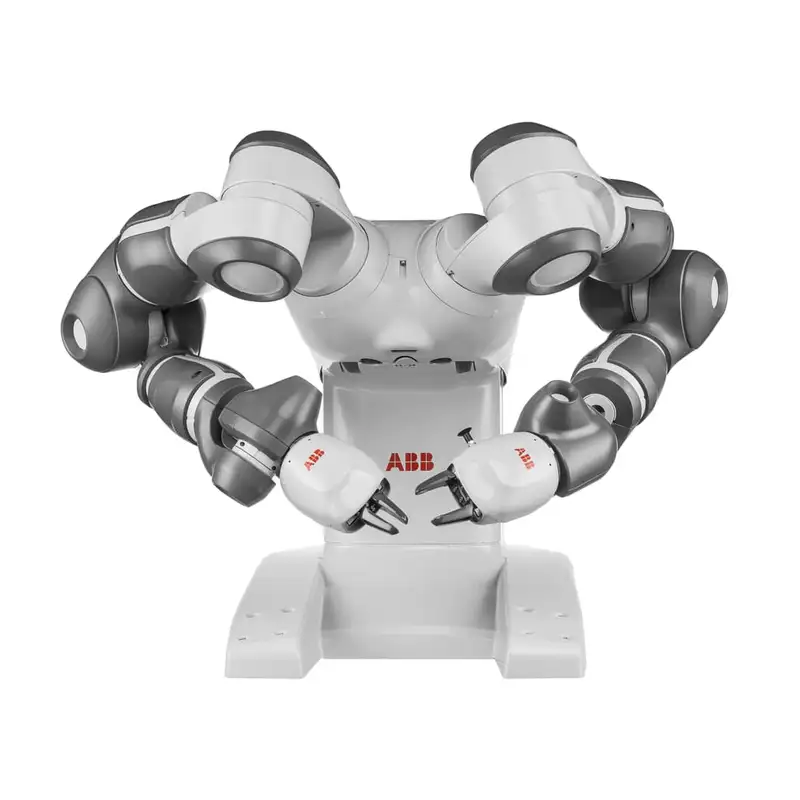
\includegraphics[scale=0.25]{figs/yumi.png}
    \caption{Dual-arm YuMi IRB 14000}
    \label{fig:dual_arm_yumi}
\end{figure}

The discussed manipulator was selected because there is URDF (Unified Robot 
Description Format) for it. However, there was no necessary representation for the 
chosen simulator. Thus, it was generated. Details is conducted later 
in Section \ref{sec:impl_details}.

\section{Frameworks}
\label{sec:frameworks}

For implementation the discussed algorithms C++ is used. Beyond of chosen language 
it is also necessary to select a simulator, a tool for computing dynamics, and 
library for solving the Gauss least constraint principle 
(\ref{eqn:least_act_principle_const}). In this section all of them is reviewed.

Firstly, let's discuss chosen simulator, MuJoCo \cite{MuJoCo}. It is general 
physical engine. In this study this framework is used to calculate system 
behavior under given control. Also, it provides way to visualize robot. From 
control point of view MuJoCo is only needed to give $\mathbf{q}$ and $\mathbf{v}$ 
at each time step. 

The system state is transferred to dynamic computing tool. This paper is utilizing 
Pinocchio \cite{Pinocchio} library. It is modern and efficient instrument for 
calculating kinematic and dynamic for given system. Notably, this frameworks 
supports the URDF, which is very convenient in the context of the selected system. 
Moreover, Pinocchio provides fast computing tools that can be further accelerated 
by code autogeneration tools. Authors of tool give the following quantities, see 
Fig. \ref{fig:pin_speed}. For implementation of proposed method this library is 
necessary only for calculating Jacobians, attitudes of frames, and velocities.

\begin{figure}[H]
    \centering
    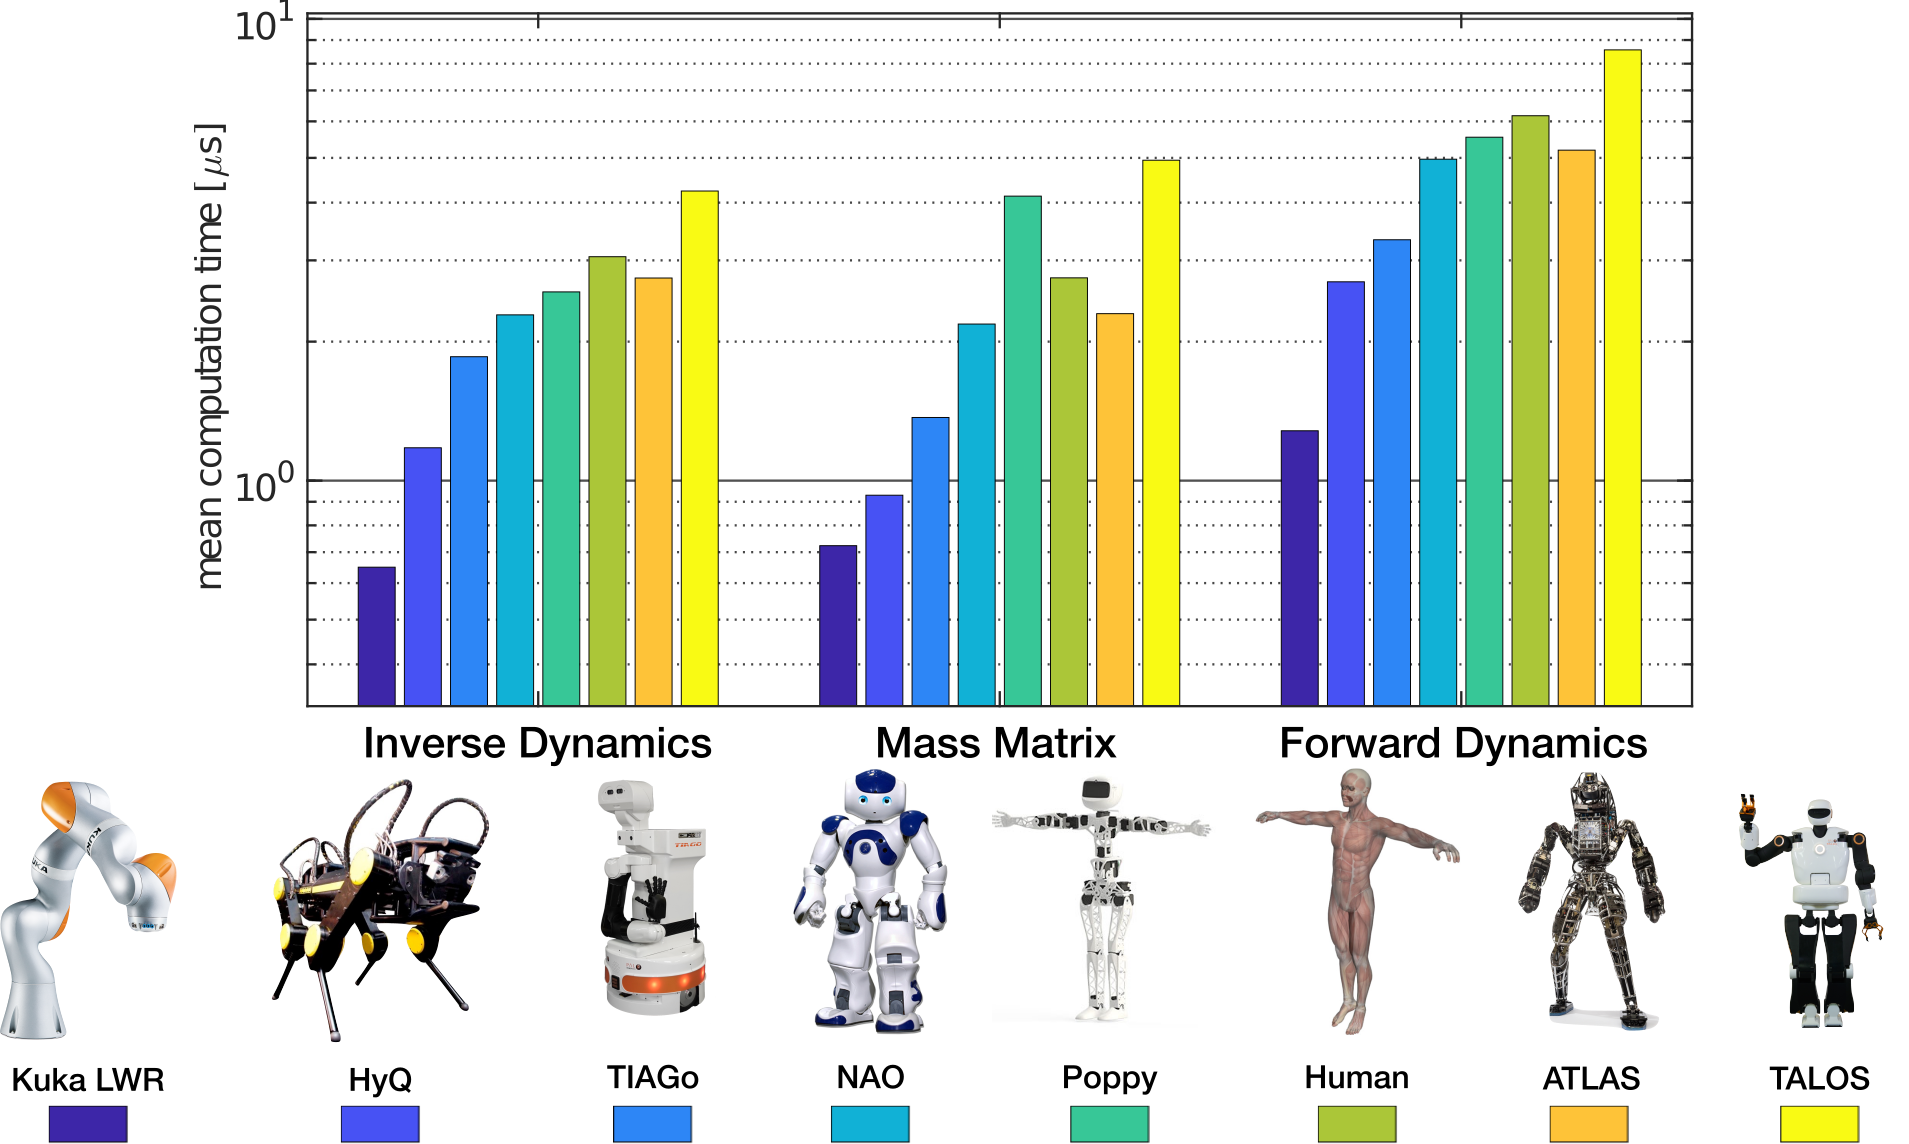
\includegraphics[scale=0.2]{figs/pin_speed.png}
    \caption{Pinocchio performance demonstration}
    \label{fig:pin_speed}
\end{figure}

Finally, the last needed element is optimization problem solver. In this paper 
ProxSuite \cite{ProxQP} is used for such purpose. The suggested methodology lies 
on quadratic problem. Authors of ProxSuite shows that their tool is fast of 
solving it. The mean computation time is 10 microseconds, see Fig. 1 in 
\cite{ProxQP}. Although, the discussed instrument is efficient but the problem 
(\ref{eqn:gauss_least_const_prior}) can be directly solved. Thus, it is needed 
to be reformulated. Further details is provided later in Section \ref{sec:impl_details}

\section{Implementation details}
\label{sec:impl_details}

This section contains details of implementation of the suggested methodology. It 
can be split into two parts, namely: computing $A$ and $\mathbf{b}$ with Pinocchio, 
and solving the problem (\ref{eqn:gauss_least_const_prior}) by ProxSuite. 
Remarkably, in this section there is no details about simulation and visualization 
because they described in MuJoCo documentation. However, it is necessary to 
mention that there is no YuMi representation for this simulator. Let's 
first discuss this moment.

The MuJoCo physical engine supports only specific XML description. It is usually 
called MJCF. For numerical experiment the total DoF was reduced to 14. Only rotation 
joints were remained. For demonstration purposes it is enough.

Now let's consider implementation of proposed algorithms 
\ref{alg:get_a_and_b}, \ref{alg:get_a_and_b_control_fixed}, and 
\ref{alg:get_a_and_b_control_rigid}. For all of them it is obligatory to compute 
Jacobians, attitude of frames, and velocities. Let's starts from system model 
and data definition:

\begin{lstlisting}[caption={Model and data}, label=snp:model_and_data]
namespace pin = pinocchio;
...
pin::Model m;
pin::urdf::buildModel("path/to/urdf", m);
pin::Data d(m);
\end{lstlisting}

Next it is necessary to compute forward kinematics for given model. As input this 
step requires generalized coordinates and velocities ($\mathbf{q}$ and 
$\mathbf{v}$). See below snippet:

\begin{lstlisting}[caption={Forward kinematics}, label=snp:forward_kin]
pin::forwardKinematics(m, d, q, v);
pin::computeJointJacobians(m, d, q);
pin::computeJointJacobiansTimeVariation(m, d, q, v);
pin::updateFramePlacements(m, d);
\end{lstlisting}

Now Jacobians, attitudes of frames, and velocities can be calculated. If $E$ is 
origin of some frame attached to system, then it has a special id in Pinocchio 
description. Let's call it \texttt{eIdx}. Thus, the code for Jacobians is

\begin{lstlisting}[caption={Jacobians}, label=snp:jacs]
using MatXd = Eigen::MatrixXd;
...
MatXd jac = MatXd::Zero(6, m.nv);
MatXd dJac = MatXd::Zero(6, m.nv);
pin::getFrameJacobian(m, d, eIdx, pin::LOCAL_WORLD_ALIGNED, jac);
pin::getFrameJacobianTimeVariation(m, d, eIdx, pin::LOCAL_WORLD_ALIGNED, dJac);
\end{lstlisting}

Here \texttt{jac} and \texttt{dJac} are Jacobian and its derivative over time 
respectively. It is important to mention that these quantities from 
$\mathbb{R}^{6 \times n_v}$. The first three rows are corresponding to 
classical linear velocity, $J_{E,v}$ or $\dot{J}_{E,v}$. The bottom three rows are 
angular part, $J_{E,\omega}$ or $\dot{J}_{E,\omega}$. All of them are expressed 
in the world coordinates.

For attitudes and velocities it is enough to execute

\begin{lstlisting}[caption={Attitudes of frames}, label=snp:atts_of_frames]
pin::Frame eFrame = m.frames[idx];
pin::FrameIndex pIdx = frame.parent;
pin::SE3 localToWorldY = pin::SE3::Identity();
localToWorldY.rotation(d.oMf[eIdx].rotation());
pin::SE3 eAtt = d.oMf[eIdx]; 
pin::Motion eVel = localToWorldY.act(frame.placement.actInv(d.v[pIdx]));
\end{lstlisting}

In snippet (\ref{snp:atts_of_frames}) \texttt{eAtt} and \texttt{eVel} are 
frame attitude and velocity respectively. \texttt{eVel} contains linear and 
angular part.

The last parts worth mentioning are the skew-symmetric operator ($[.]^{\wedge}$) 
and matrix logarithm ($\log (.)$). In Pinocchio they are \texttt{pin::skew} and 
\texttt{pin::log3} function respectively. Other mathematical operations are not 
worth to be explained due to their triviality. 

All snippets above are used for experiment. They can be found in the repository 
\cite{experimentsRepo}. However, for optimization and readability they 
are realized not in the same order. Also for the same purposes, auto-generation is 
not used in this example. In the provided code algorithm 
\ref{alg:get_a_and_b} is demonstrated in \texttt{getConstraintsAffineDesc}, 
algorithm \ref{alg:get_a_and_b_control_fixed} is shown in \\
\texttt{getControlAffineDesc}, the last one \ref{alg:get_a_and_b_control_rigid} 
can be implemented by function \\ \texttt{getAffineDesc}. Again, see 
\cite{experimentsRepo}.

Now let's discuss the transformation of equation 
(\ref{eqn:gauss_least_const_prior}) for ProxSuite framework. This library can 
handle quadratic problem of the following form

\begin{equation}
    \begin{aligned}
        \min_{\mathbf{x}} \quad & 
        \frac{1}{2} \mathbf{x}^T H \mathbf{x} + 
        \mathbf{g}^T \mathbf{x} \\
        \textrm{s.t.} \quad & A \mathbf{x} = \mathbf{b} \\
        & \mathbf{y}_l \leq C \mathbf{x} \leq \mathbf{y}_u  
    \end{aligned}
    \label{eqn:prox_qp_form}
\end{equation}

where $[.] \leq [.]$ is element-wise vector operator, $H \succeq 0$, and 
other quantities are arbitrary.

In case of the Gauss least constraint principle the last line of quadratic 
problem (\ref{eqn:prox_qp_form}) is unnecessary. Hence, it is enough 
to open brackets of equation (\ref{eqn:gauss_least_const_prior}):

\begin{equation}
    \begin{aligned}
        \min_{\dot{\mathbf{v}}} \quad & 
        \frac{1}{2} \dot{\mathbf{v}}^T [M + \omega A_u^T A_u] \dot{\mathbf{v}} + 
        [-\mathbf{Q} - \omega A_u^T \mathbf{b}_u]^T \dot{\mathbf{v}} \\
        \textrm{s.t.} \quad & A_c \dot{\mathbf{v}} = \mathbf{b}_c
    \end{aligned}
    \label{eqn:gauss_least_const_to_prox_qp}
\end{equation}

The removing of unconstrained acceleration $\mathbf{a}$ is possible by equation 
(\ref{eqn:can_man_eqn_simple}). Thus, $H = M + \omega A_u^T A_u$ and 
$\mathbf{g} = -\mathbf{Q} - \omega A_u^T \mathbf{b}_u$. The problem 
(\ref{eqn:gauss_least_const_to_prox_qp}) is solvable by the following 
code

\begin{lstlisting}[caption={Quadratic problem solution}, label=snp:qp_sol]
namespace prox = proxsuite::proxqp;
...
prox::dense::QP<double> qp(m.nv, 6, 0);
qp.settings.eps_abs = eps_abs;
qp.settings.initial_guess = prox::InitialGuessStatus::NO_INITIAL_GUESS;
qp.settings.verbose = false;
qp.init(
    M + omega * Au.transpose() * Au,
    -Q - omega * Au.transpose() * bu,
    Ac, bc,
    proxsuite::nullopt, proxsuite::nullopt, proxsuite::nullopt
);
qp.solve();
\end{lstlisting}

After first computation it is recommended to use \\
\texttt{prox::InitialGuessStatus::WARM\_START} to speed up calculation. This 
flag enables initial guess taken from previous solution.

\section{Simulation results}
\label{sec:sim_results}

During the experiment the following presets for YuMi are following

\begin{longtable}{|p{.30\textwidth}|l|}
\hline
Quantity & Used in experiment \\ 
\hline
Frame $\mathcal{E}_1$ & Joint frame \texttt{yumi\_link\_7\_l} in URDF \\ 
\hdashline
Frame $\mathcal{E}_2$ & Joint frame \texttt{yumi\_link\_7\_r} in URDF \\ 
\hdashline
$T_{\mathcal{A}}^{\mathcal{B}}$ & 
$\begin{bmatrix}
    1 & 0 & 0 & 0 \\
    0 & 0 & 1 & -0.4 \\
    0 & -1 & 0 & 0.12 \\
    0 & 0 & 0 & 1  
\end{bmatrix}$ \\
\hdashline
Constraint $K_p$ & 1000 \\
\hdashline
Constraint $K_d$ & 33 \\ 
% \hline
Control $K_p$ & 500 \\ 
\hdashline
Control $K_d$ & 17 \\ 
\hdashline
$\omega$ from equation (\ref{eqn:gauss_least_const_prior}) & 50 \\ 
\hdashline
Desired law ($T_{\mathcal{W}}^{\mathcal{D}}$) of motion for $\mathcal{E}_1$ & 
$\begin{bmatrix}
    1 & 0 & 0 & 0.436763 + 0.12 \cdot \cos(1.5 t + \pi / 2) \\
    0 & 1 & 0 & 0.185684 \\
    0 & 0 & 1 & 0.512661 + 0.12 \cdot \sin(1.5 t + \pi / 2) \\
    0 & 0 & 0 & 1
\end{bmatrix}$ \\ 
\hdashline
Initial $\mathbf{q}$ & See in \cite{experimentsRepo} \\ 
\hdashline
Initial $\mathbf{v}$ & $\mathbf{0}$ \\ 
\hline
\end{longtable}

The initial $\mathbf{q}$ is around of ideal one that gives zero control and 
constraint error. Simulation shows the following behavior of generalized 
coordinates and velocities under proposed control, see Fig. \ref{fig:q_and_v_plot}

\begin{figure}[H]
    \centering
    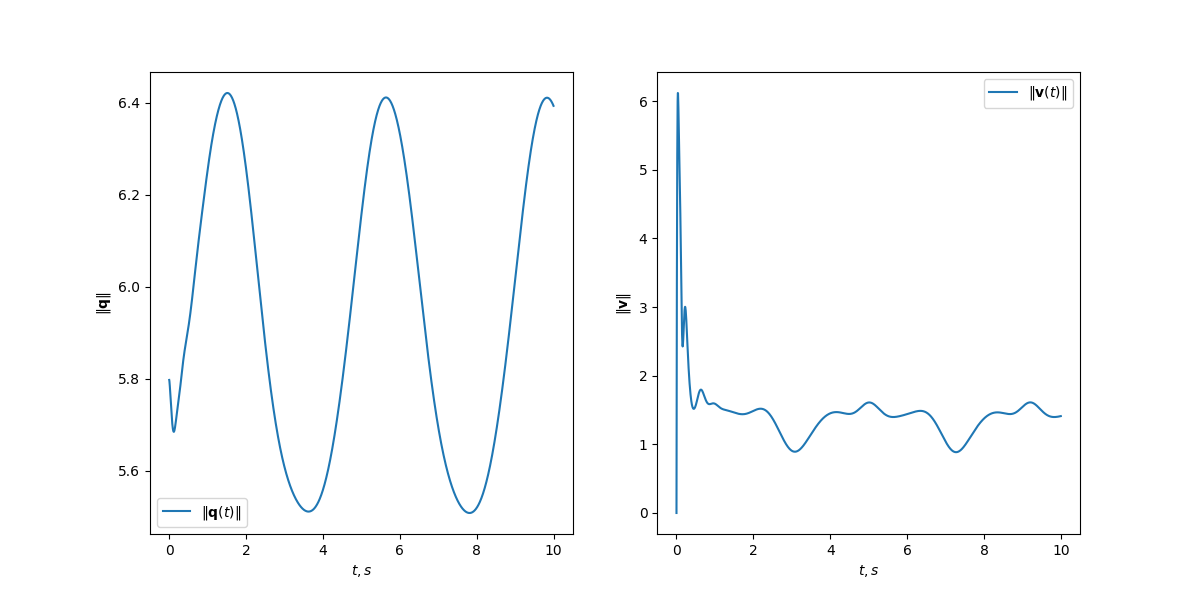
\includegraphics[scale=0.52]{figs/q_and_v_history.png}
    \caption{Experimental $\mathbf{q}$ and $\mathbf{v}$}
    \label{fig:q_and_v_plot}
\end{figure}

The plot of $\|\mathbf{q}\|$ and $\|\mathbf{v}\|$ over time demonstrates 
convergence to some periodical function. It can be explained by chosen 
desired law with period $4 \pi / 3$. Although, it is indirect proof of success, but 
the plot of positions shows stability of proposed methodology, see Fig. 
\ref{fig:poses_plot}. Subscript $s$ stands for $\mathcal{E}_1$ frame, 
and $e$ stands for $\mathcal{E}_2$.

\begin{figure}[H]
    \centering
    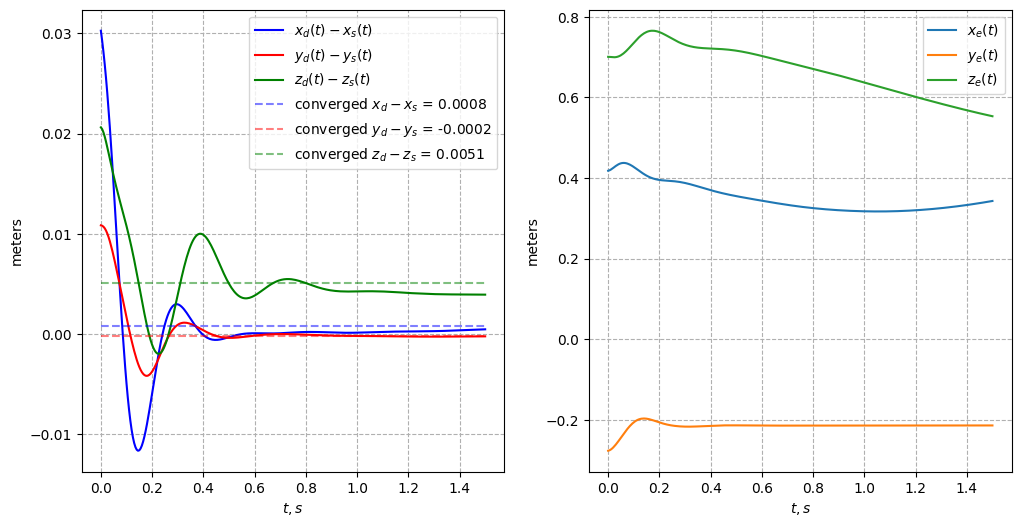
\includegraphics[scale=0.52]{figs/poses_history.png}
    \caption{Experimental frame positions}
    \label{fig:poses_plot}
\end{figure}

\begin{figure}[H]
    \centering
    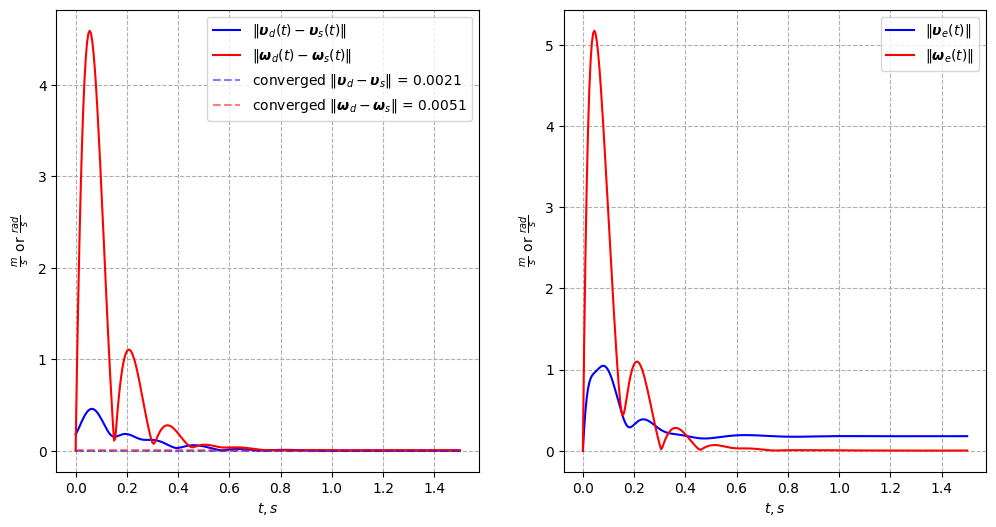
\includegraphics[scale=0.52]{figs/vels_history.png}
    \caption{Experimental frame velocities}
    \label{fig:vels_plot}
\end{figure}

The graph of difference between desired position and actual one converges to 
zero with some numerical noise. In Fig. \ref{fig:poses_plot} the obtained 
values are mean after $t > 1.5$. The steady state response time is less 
than $0.75$ second according to Fig. \ref{fig:vels_plot}. Futhermore, 
the $\mathbf{e}_{\SE}$ for constraint converges faster, see  
Fig. \ref{fig:errors_plot}. However, control error converges to zero 
same as velocities.

\begin{figure}[H]
    \centering
    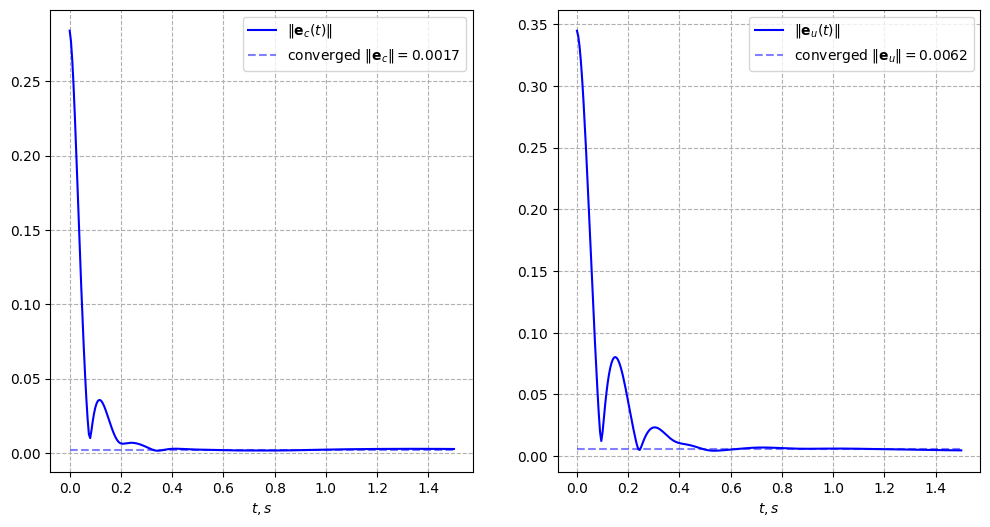
\includegraphics[scale=0.52]{figs/errors_history.png}
    \caption{Experimental $\mathbf{e}_{\SE}$, left $\mathbf{e}_c$ - constraint, 
    right $\mathbf{e}_u$ - control}
    \label{fig:errors_plot}
\end{figure}

The obtained results of numerical experiment proves the workability 
of suggested methodology. Nevertheless, results does not demonstrate convergence 
of over-damped system. Thus, finetuning of $K_p$, $K_d$ is still needs 
further investigations.

\chapter{Evaluation and Discussion}
\label{chap:eval}

\chapter{Conclusion}
\label{chap:conclusion}


\appendix
\chapter{Brief Lie theory}

The Lie group, a mathematical concept dating back to the 19th century, was 
first proposed by Sophus Lie, laying the foundation for continuous 
transformation groups. Although it was initially abstract, over time its 
influence has spread to various scientific and technological fields. The 
mathematical tools discussed in this chapter are crucial for the research 
discussed here. It inspired by this study \cite{MicroLieTheory}, and 
contains only crucial information.

\section{Groups, Algebras, and operators}
\label{sec:group_algebra_ops}

Let $\mathcal{G}$ is smooth manifold that satisfies the group axioms. For any 
$\mathcal{X}$, $\mathcal{Y}$ and $\mathcal{Z}$ from $\mathcal{G}$ the following 
statements are true:

\begin{equation}
    \begin{aligned}
        \label{eqn:g_axi}
        & \mathcal{X} \circ \mathcal{Y} \in \mathcal{G} \quad && \text{(I)} \\
        & \exists \mathcal{E}:\ \mathcal{E} \circ \mathcal{X} 
        = \mathcal{X} \circ \mathcal{E} = \mathcal{X} \quad && \text{(II)} \\
        & \exists \mathcal{X}^{-1}:\ \mathcal{X}^{-1} \circ \mathcal{X}
        = \mathcal{X} \circ \mathcal{X}^{-1} = \mathcal{E} \quad && \text{(III)} \\ 
        & (\mathcal{X} \circ \mathcal{Y}) \circ \mathcal{Z} = 
        \mathcal{X} \circ (\mathcal{Y} \circ \mathcal{Z}) \quad && \text{(IV)}
    \end{aligned}
\end{equation}

For such group $T_{\mathcal{E}} \mathcal{G}$ is the Lia Algebra defined at 
$\mathcal{E}$ element. The geometric interpretation of algebra is tangent plane 
that touches the smooth manifold (group). $\mathfrak{m} \equiv 
T_{\mathcal{E}} \mathcal{G}$ is always a vector space.

The next crucial definition is a group action

\begin{equation}
    f: \mathcal{G} \times \mathcal{V} \to \mathcal{V}
\end{equation}

where $\mathcal{V}$ is some set. The operation defined above should satisfy 
the axioms ($v \in \mathcal{V}$; $\mathcal{X}, \mathcal{Y} \in \mathcal{G}$),

\begin{equation}
    \begin{aligned}
        \label{eqn:act_axi}
        & \mathcal{E} \cdot v = v \quad && \text{(I)} \\
        & (\mathcal{X} \circ \mathcal{Y}) \cdot v = 
        \mathcal{X} \cdot (\mathcal{Y} \cdot v) \quad && \text{(II)}
    \end{aligned}
\end{equation}

For instance, if the $\text{SO}(n)$ rotations is considered as Lie group, than the 
transformation $R \cdot x \equiv R x$ ($x \in \mathbb{R}^n$) is a group action.

The exponential map $\exp:\ \mathfrak{m} \to \mathcal{G}$ converts elements of 
Lie algebra to corresponding group. The log map do inverse operation. 
However, it is necessary to remember that 
this map applicable only for "identity" algebra. However, there is a linear
transformation between $T_{\mathcal{X}} \mathcal{G}$ and $T_{\mathcal{E}} 
\mathcal{G}$. It is called adjoin.

It is known that $\mathfrak{m}$ is isomorphic to the vector space $\mathbb{R}^m$. 
One can write it as $\mathfrak{m} \cong \mathbb{R}^m$. Due to convenience this 
isomorphism would be highly utilized. Moreover, in the bellow sections only 
algebras constructed on $\mathbb{R}^m$ are considered. Thus, a mapping between 
sets can be defined in the following manner (hat-vee notation)

\begin{equation}
    \begin{aligned}
        \label{eqn:hat_vee_not}
        & [*]^\wedge: \ \mathbb{R}^m \to \mathfrak{m} \quad &&
        \boldsymbol{\tau}^\wedge = \sum_{i=1}^{m} \tau_i E_i \\
        & [*]^\vee: \mathfrak{m} \to \mathbb{R}^m \quad && 
        \boldsymbol{\tau} = \sum_{i=1}^{m} \tau_i \mathbf{e}_i
    \end{aligned}
\end{equation}

where $\mathbf{e}_i$ are a base of $\mathbb{R}^m$ and $E_i$ are base vectors 
of $\mathfrak{m}$. Obviously, $\mathbf{e}_i^\wedge = E_i$. Using this mapping, the
exponential / log map can be modified 

\begin{equation}
    \begin{aligned}
        \label{eqn:exp_log_for_r_m}
        & \exp : \quad && \mathcal{X} = \exp(\boldsymbol{\tau}^\wedge) \\
        & \log : \quad && \boldsymbol{\tau} = \log(\mathcal{X})^\vee
    \end{aligned}
\end{equation}

Or, in the most convenient form

\begin{equation}
    \begin{aligned}
        \label{eqn:big_exp_log_for_r_m}
        & \text{Exp} : \quad && \mathcal{X} 
        = \exp(\boldsymbol{\tau}^\wedge) 
        = \text{Exp}(\boldsymbol{\tau})\\
        & \text{Log} : \quad && \boldsymbol{\tau} 
        = \log(\mathcal{X})^\vee
        = \text{Log}(\mathcal{X})
    \end{aligned}
\end{equation}

Through this definitions it easy to introduce plus and minus operations

\begin{equation}
    \begin{aligned}
        & \text{right-} \oplus: &&
        \mathcal{X} \oplus \prescript{\mathcal{X}}{}{\boldsymbol{\tau}} 
        \equiv \mathcal{X} \circ 
        \text{Exp}(\prescript{\mathcal{X}}{}{\boldsymbol{\tau}}) \in 
        \mathcal{G} \\
        & \text{right-} \ominus: &&
        \mathcal{Y} \ominus \mathcal{X} 
        \equiv \text{Log}(\mathcal{X}^{-1} \circ \mathcal{Y}) 
        \in T_{\mathcal{X}}\mathcal{G} \\
        & \text{left-} \oplus: &&
        \prescript{\mathcal{E}}{}{\boldsymbol{\tau}} \oplus \mathcal{X}
        \equiv \text{Exp}(\prescript{\mathcal{E}}{}{\boldsymbol{\tau}}) 
        \circ \mathcal{X} \in \mathcal{G} \\ 
        & \text{left-} \ominus: &&
        \mathcal{Y} \ominus \mathcal{X} \equiv
        \text{Log}(\mathcal{Y} \circ \mathcal{X}^{-1}) 
        \in T_{\mathcal{E}}\mathcal{G}
    \end{aligned}
\end{equation}

Using the above statements it is possible to define Jacobians

\begin{equation}
    \begin{aligned}
        & J_r(\boldsymbol{\tau}): &&
        \text{Exp}(\boldsymbol{\tau} + \delta \boldsymbol{\tau})
        \approx
        \text{Exp}(\boldsymbol{\tau}) \oplus 
        [J_r(\boldsymbol{\tau}) \delta \boldsymbol{\tau}] \\ 
        & J_r^{-1}(\boldsymbol{\tau}): &&
        \text{Log}(\mathcal{X} \oplus \delta \boldsymbol{\tau}) 
        \approx
        \text{Log}(\mathcal{X}) + 
        J_r^{-1}(\boldsymbol{\tau}) \delta \boldsymbol{\tau}
    \end{aligned}
\end{equation}

where $\mathcal{X} = \text{Exp}(\boldsymbol{\tau})$, and $\oplus$, $\ominus$ 
are right versions. The above definitions describe right version of 
Jacobians. There are also left ones that based on left minus and plus 
operators.

\section{Special orthogonal group}

Let's consider $\SO$ (Special orthogonal group). It consists from orthogonal 
rotations matrices, and forms a group under multiplication. According to 
Euler's rotation theorem any orientation can be described by rotation 
about some single axis with precision to $2 \pi n$. Thus, $\SO$ can be 
considered as Lie group, and $\mathbb{R}^3$ is a Lie algebra respectively.

Now let's define a wedge operator $[.]^{\wedge}$:

\begin{equation}
    \hat{\mathbf{a}} = \mathbf{a}^{\wedge} = 
    \begin{bmatrix}
        0 & -a_3 & a_2 \\
        a_3 & 0 & -a_1 \\
        -a_2 & a_1 & 0 \\
    \end{bmatrix}
    \label{eqn:wedge_op}
\end{equation}

where $\mathbf{a} \in \mathbb{R}^3$, and vee operator ($[.]^{\vee}$) is 
following

\begin{equation}
    A^{\vee} = \mathbf{a}, \ \text{where }
    \hat{\mathbf{a}} = A
    \label{eqn:vee_op}
\end{equation}

Using these definitions it is possible to connect $\dot{R}$ with classical 
angular velocity

\begin{equation}
    \begin{aligned}
        \hat{\boldsymbol{\omega}}^s = \dot{R} R^T & \quad
        \hat{\boldsymbol{\omega}}^b = R^T \dot{R}
    \end{aligned}
    \label{eqn:ang_with_dot_r}
\end{equation}

where $b$ and $s$ subscripts denote body and spatial velocities 
respectively.

The exponential map is

\begin{equation}
    R = \text{Exp}(\boldsymbol{\theta}) \equiv
    I + \frac{\sin \theta}{\theta} \hat{\boldsymbol{\theta}} +
    \frac{1 - \cos \theta}{\theta^2} \hat{\boldsymbol{\theta}}^2
    \label{eqn:exp_map}
\end{equation}

where $\boldsymbol{\theta} = \theta \mathbf{u}$, and $\mathbf{u}$ is 
arbitrary unit vector from $\mathbb{R}^3$. Therefore, the logarithm map is

\begin{equation}
    \boldsymbol{\theta} = \text{Log}(R) \equiv 
    \frac{\theta (R - R^T)^{\vee}}{2 \sin \theta}, \ 
    \text{where } 
    \theta = \cos^{-1} \frac{\text{trace}(R) - 1}{2}
    \label{eqn:log_map}
\end{equation}

In the above statement $R - R^T$ is skew symmetric, it can be proved by 
transposing it. 

Now let's move to left and right Jacobians definitions 

\begin{equation}
    \begin{aligned}
        J_r(\boldsymbol{\theta}) & = 
        I - \frac{1 - \cos \theta}{\theta^2} \hat{\boldsymbol{\theta}} +
        \frac{\theta - \sin \theta}{\theta^3} \hat{\boldsymbol{\theta}}^2 \\
        J_r^{-1}(\boldsymbol{\theta}) & = 
        I + \frac{1}{2} \hat{\boldsymbol{\theta}} + 
        \biggl( \frac{1}{\theta^2} - 
        \frac{1 + \cos \theta}{2 \theta \sin \theta} \biggr)
        \hat{\boldsymbol{\theta}}^2 \\ 
        J_l(\boldsymbol{\theta}) & = J_r^T(\boldsymbol{\theta}) \\
        J_l^{-1}(\boldsymbol{\theta}) & = J_r^{-T}(\boldsymbol{\theta})
    \end{aligned}
    \label{eqn:l_and_r_jacobians}
\end{equation}

The all of the above definitions are reformulated from Appendix B in 
\cite{MicroLieTheory}. The mathematical ground for them can be found 
in \cite{LieStochModels}.


%% REFERENCES
\printbibliography[heading=bibintoc,title={Bibliography cited}]
\end{document}
